% \section{Introduction}
% Empty subsection to make a blank space in headline
% \subsection{}

% \begingroup
% \setbeamertemplate{navigation symbols}{}  % remove page number within the group
% \begin{frame}[noframenumbering, plain]{\ }
% \hfill
% \parbox[t]{.85\textwidth}{
%   \begin{minipage}[c][0.65\textheight]{\textwidth}
%   \tableofcontents[currentsection, subsectionstyle=show/shaded/shaded]
%   \end{minipage}
% }
% \end{frame}
% \endgroup

\begingroup
    \setbeamertemplate{headline}{}

\begin{frame}{Introduction}
\begin{minipage}[t]{0.5\linewidth}
    \vspace{0pt}
        \centering\textbf{General context}
        \begin{itemize}
            \item Elderly population is growing
            \item Higher levels of frailty globally
            \item Increasing demand for reliable monitoring devices
            \item Tarkett, French company: 12,500 employees, 13 industrial sites, 1.3 millions m$^2$ of flooring per day
            \item \emph{Floor in Motion}: a floor-based sensor for elderly care
            \item \textbf{Objective}: providing tools for elderly monitoring in nursing homes
        \end{itemize}
            \smallskip
            \onslide<2->
\includegraphics[width=0.4\linewidth]{FIM.jpg}\\[2pt]
            \onslide<2->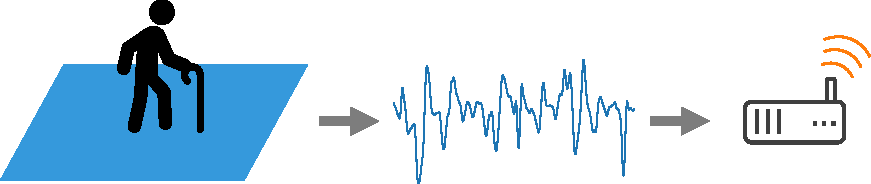
\includegraphics[width=0.95\linewidth]{schema_fall_detector.pdf}\\
    \pause \pause
\end{minipage}\hfill
\begin{minipage}[t]{0.49\linewidth}
        \vspace{0pt}
        \centering\textbf{Scientific context}
        \begin{itemize}
            \item Processing and understanding time series
    %         \begin{itemize}
    %             \item Proliferation of sensor-based systems
    %             \item Redundancy, interpretability, external pertubations
    %         \end{itemize}
            \item Real world application
    %         \begin{itemize}
    %             \item Real-time processing in a limited system
    %             \item Convenient hypotheses not granted
    %         \end{itemize}
        \end{itemize}
%         \begin{figure}[h]
%                 \centering
%                 \vspace{0.5cm}
%                 \onslide<2->
\includegraphics[width=0.4\linewidth]{Tarkett-logo_red.jpg}\\[5pt]
%                 \pause
        %         \onslide<2->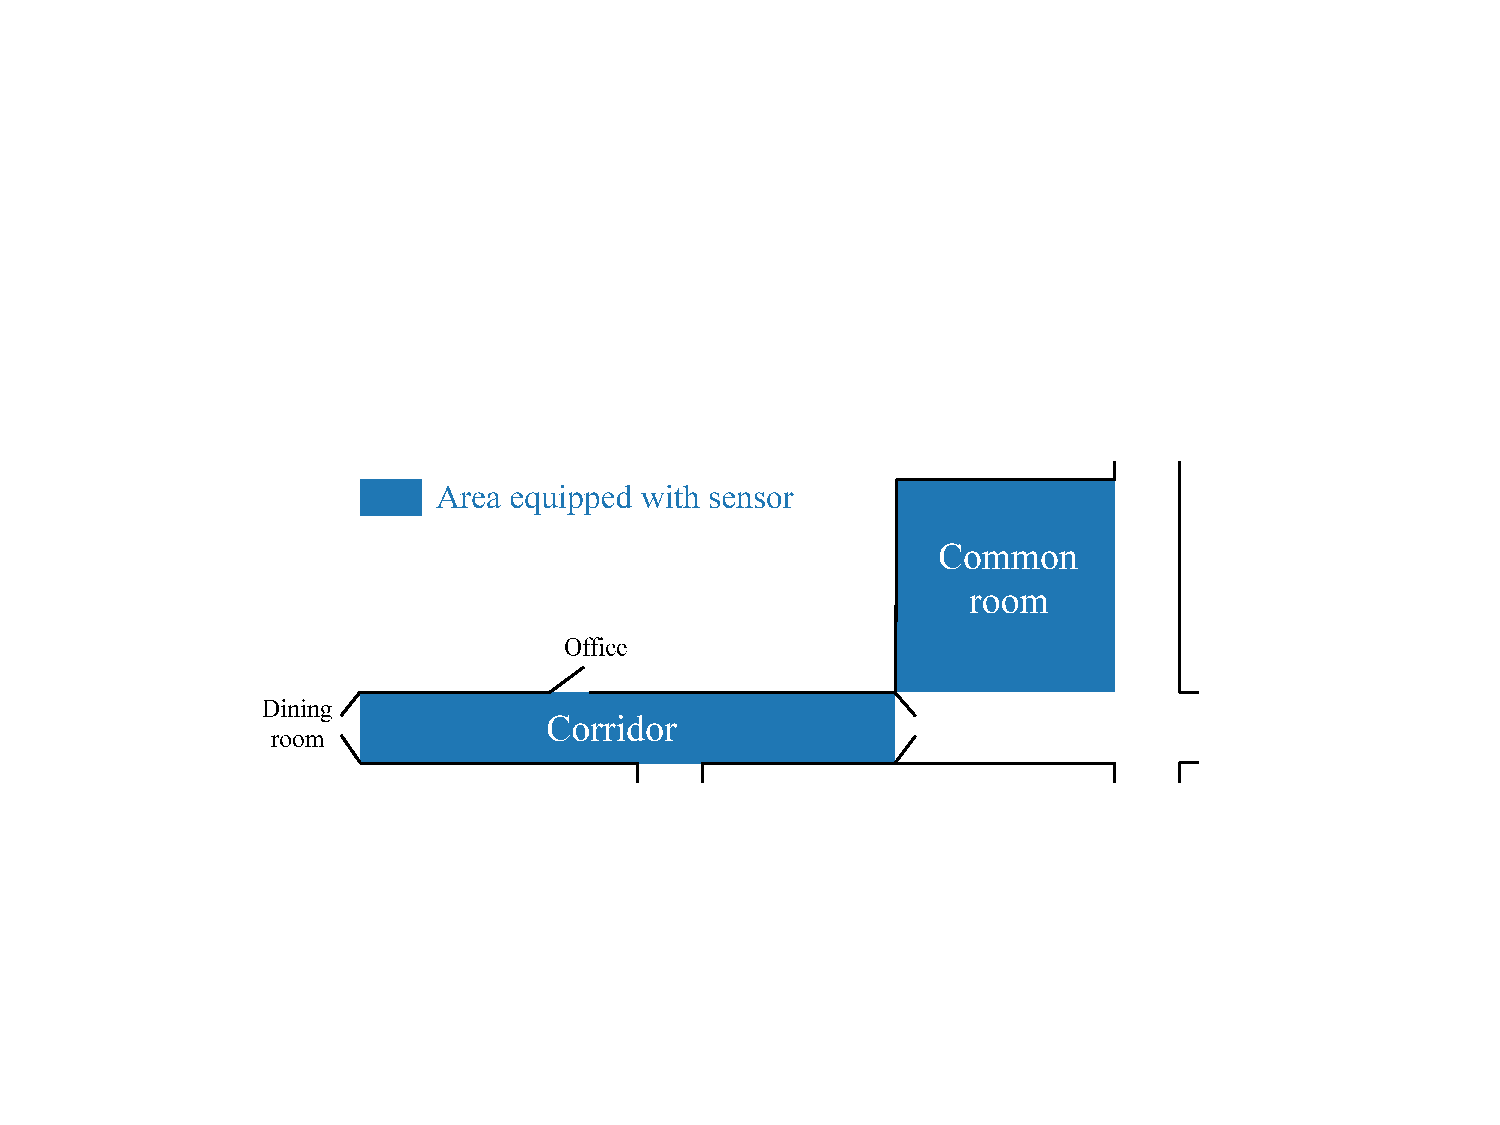
\includegraphics[width=0.6\linewidth, trim= 50 150 50 210, clip]{schema_couloir_plan_blue.pdf}
        %     \end{minipage}
        %     \caption{System installation in a nursing home.}
        %     \label{fig:schema_installation}
%         \end{figure}
%     \bigskip
        \centering
        \begin{minipage}[t]{0.45\linewidth}
            \vspace{0.5pt}
            \centering
            \onslide<3->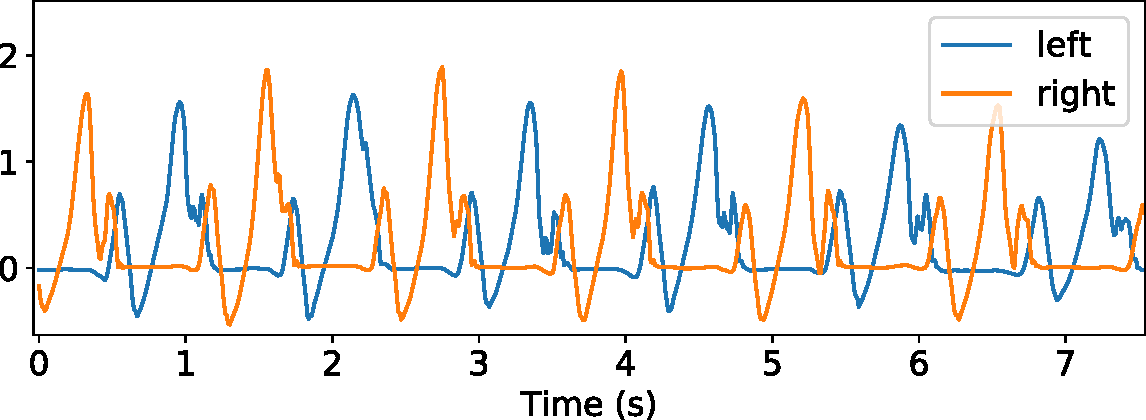
\includegraphics[width=0.91\linewidth]{signal_marche_accelerometre_left_right_epure.pdf}\\
            {\small Foot-attached accelerometer}
        \end{minipage}
        \begin{minipage}[t]{0.45\linewidth}
            \vspace{0pt}
            \centering
            \onslide<3->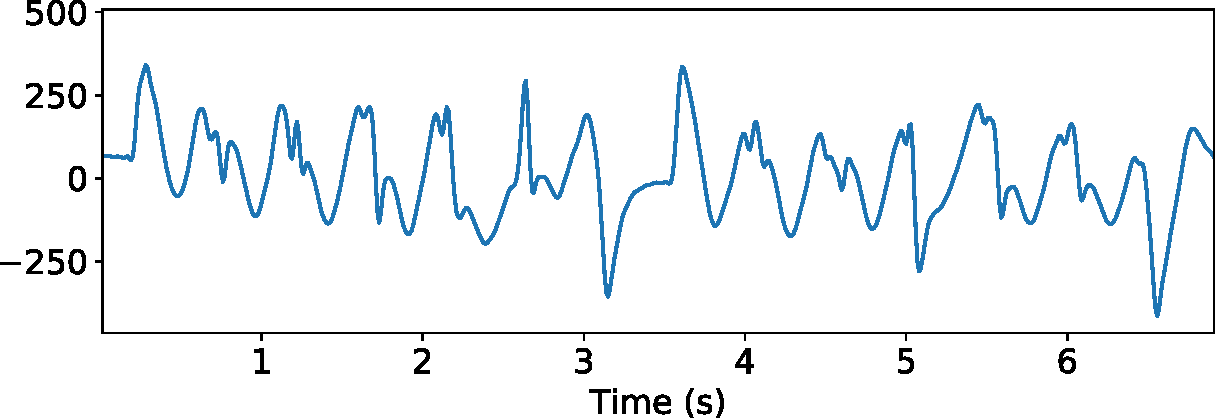
\includegraphics[width=\linewidth]{signal_marche_tarkett_epure.pdf}\\
            {\small Tarkett's floor sensor}
        \end{minipage}
        
    \pause
    \medskip
    \centering\textbf{Questions}
    \begin{itemize}
        \item Is a floor-based system a good idea ?
        \item How to build a fall detector out of it ?
        \item How to use real data to improve our model ?
        \item The signal is unidimensional: can we still distinguish people ?
    \end{itemize}
\end{minipage}
\end{frame}

\endgroup

% Outline
\begingroup
\setbeamertemplate{headline}{}
\setbeamertemplate{navigation symbols}{}  % remove page number within the group
\setcounter{tocdepth}{1}
\begin{frame}[noframenumbering]{Table of contents}
% \parbox[t]{.85\textwidth}{
%     \begin{minipage}[c][0.65\textheight]{\textwidth}
    \centering
%     \vspace{1.0cm}
    \large
    \tableofcontents
%     \end{minipage}
% }
\end{frame}
\endgroup

\section{Monitoring systems}

\begin{frame}{}
    \centering
    \vspace{3cm}
    \Huge
    \textcolor{myblue}{Monitoring systems for fall detection}
\end{frame}


\subsection{Sensors}

\begin{frame}{Sensors}{}
    
    \begin{minipage}[t]{0.49\linewidth}
        \vspace{0pt}
What makes a good monitoring system ?
        \begin{itemize}
            \item coverage and occlusion
            \item intrusiveness
            \item signal quality / information
            \item robustness
            \item ease of installation / use
            \item scalability
        \end{itemize}

    \end{minipage}\hfill
    \begin{minipage}[t]{0.49\linewidth}
        \vspace{0pt}
        \begin{overprint}
            \onslide<2>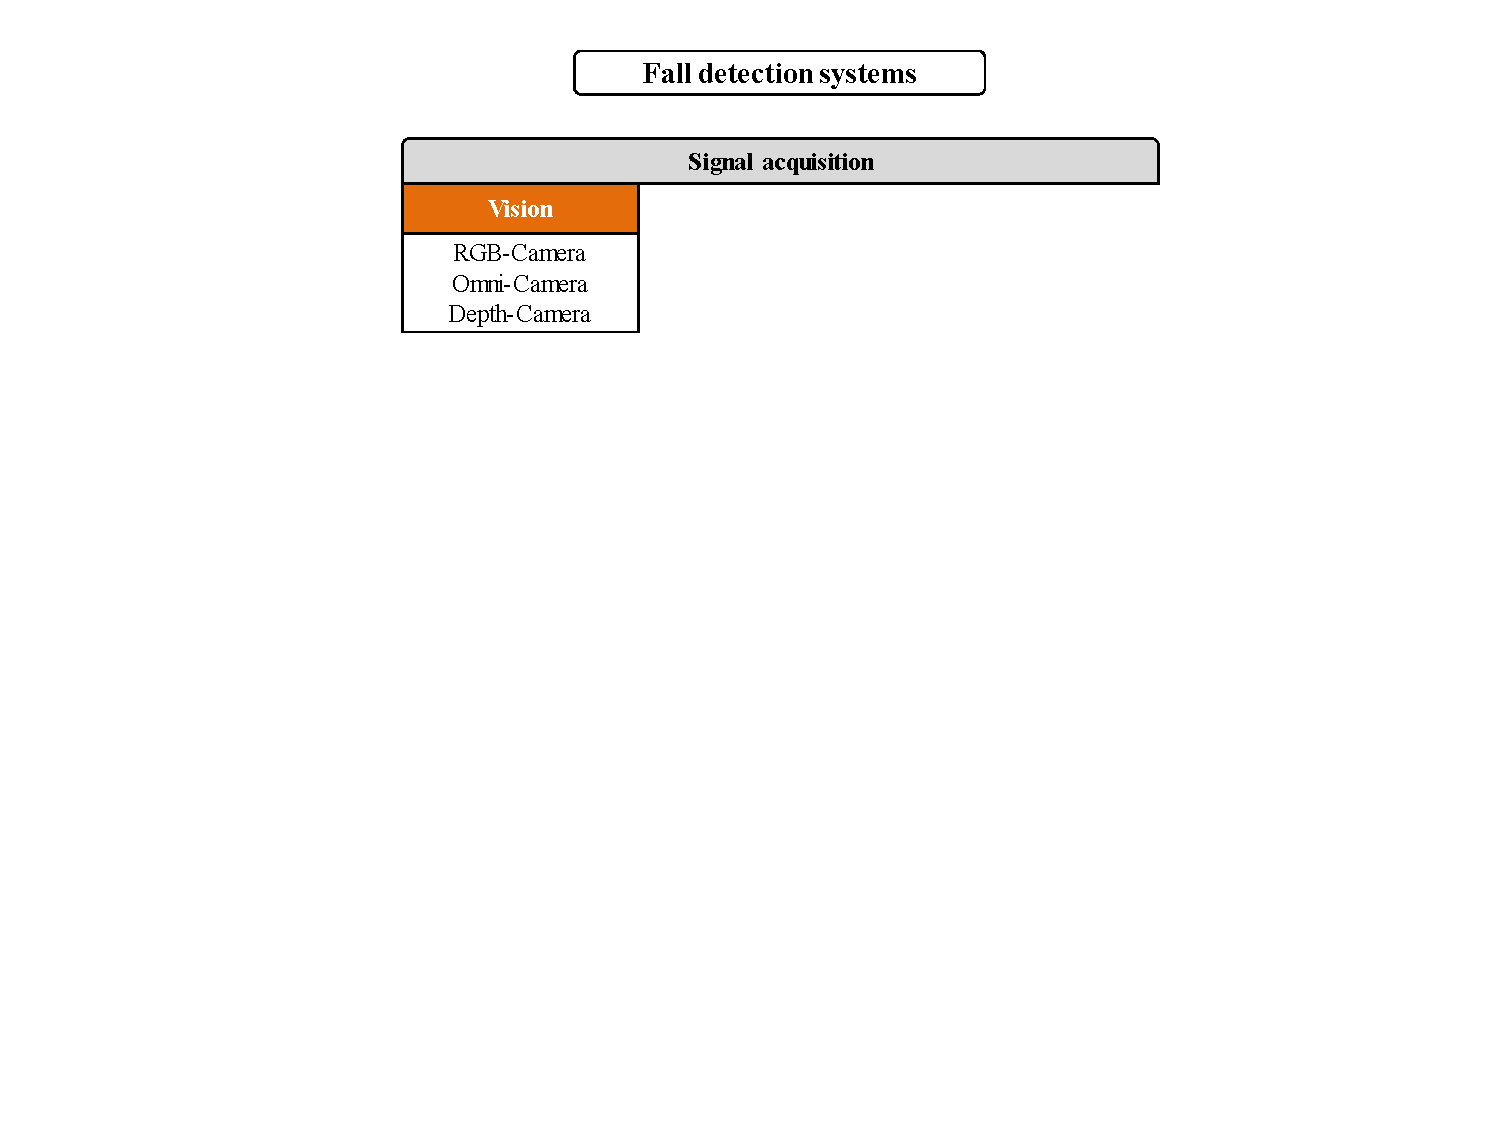
\includegraphics[width=\linewidth, trim={190 250 150 60}, clip]{fall_systems_1_1-14.pdf}
            \onslide<3>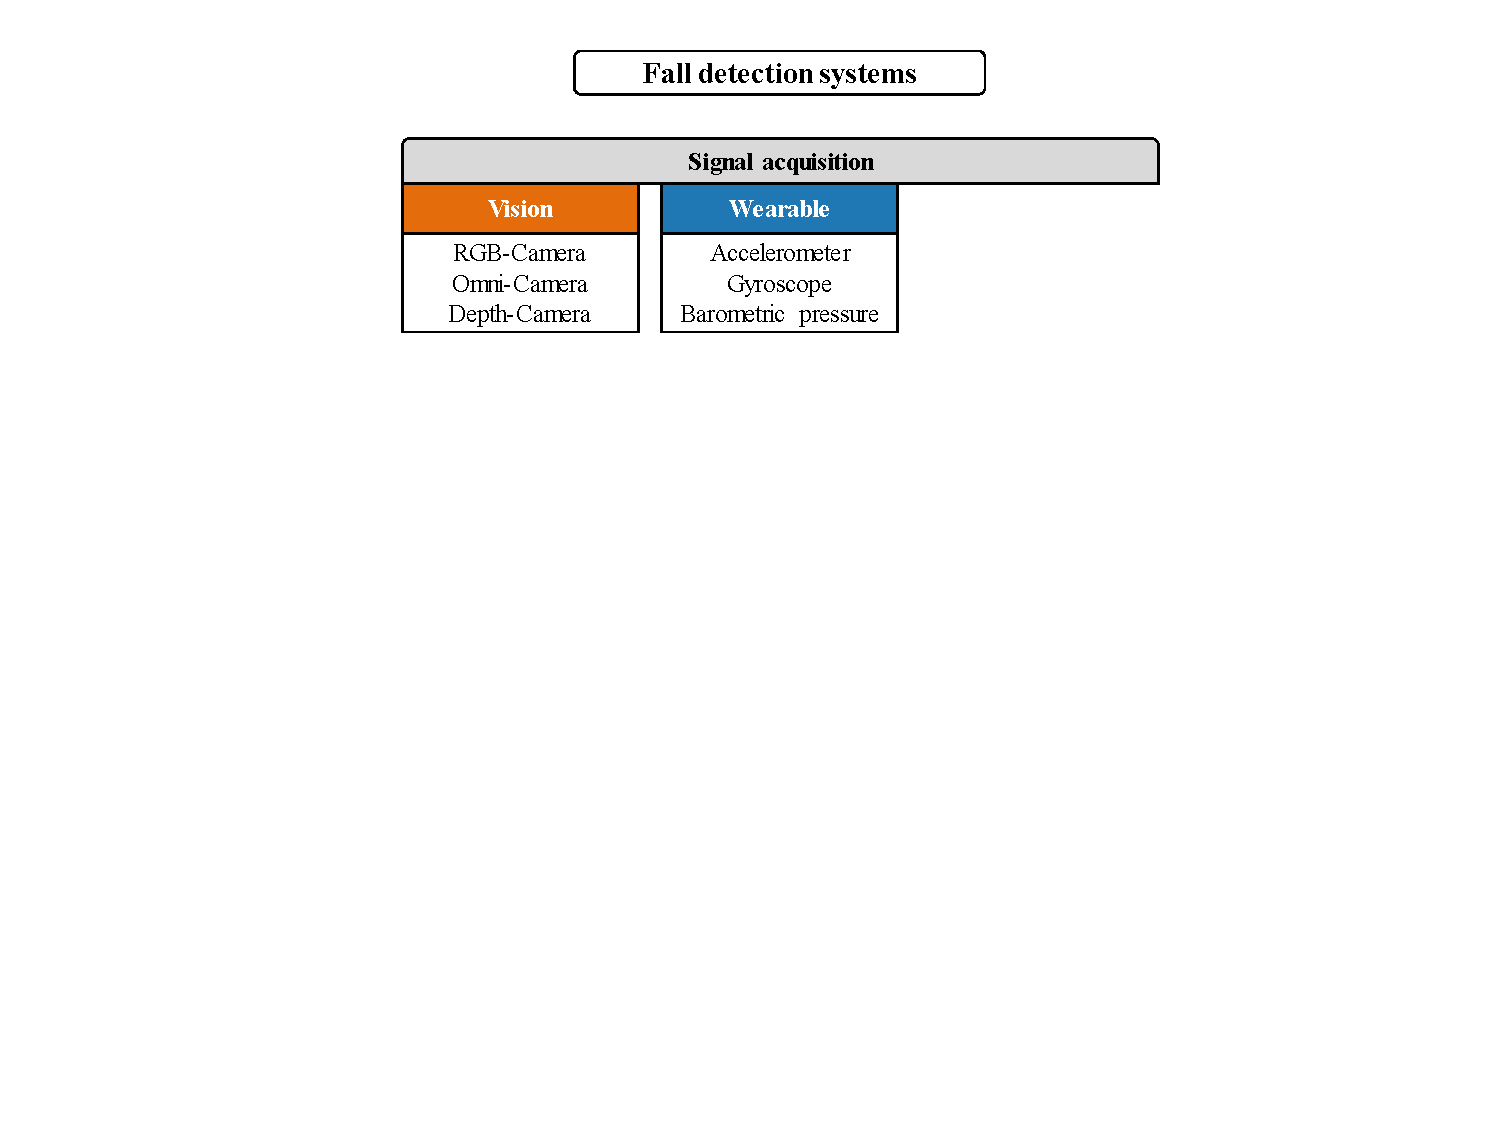
\includegraphics[width=\linewidth, trim={190 250 150 60}, clip]{fall_systems_1_2-14.pdf}
            \onslide<4>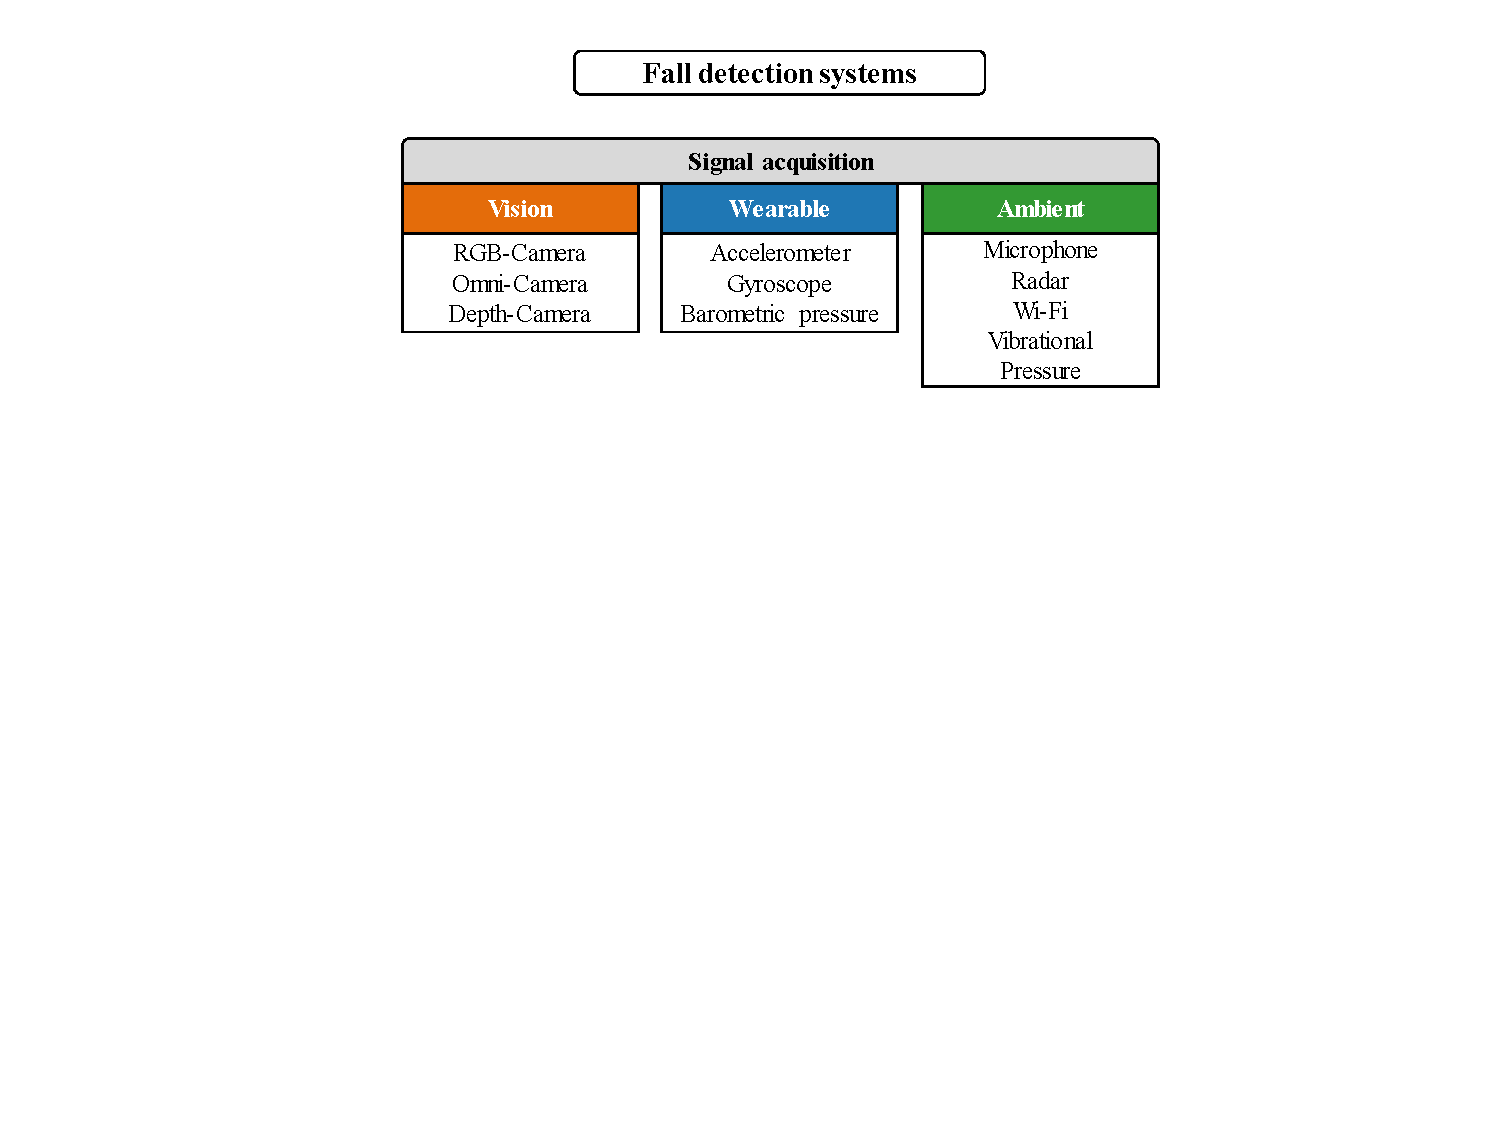
\includegraphics[width=\linewidth, trim={190 250 150 60}, clip]{fall_systems_1_3-14.pdf}
        \end{overprint}
    \end{minipage}
% \end{minipage}

\vspace{-0.8cm}
% \onslide<1>{
\renewcommand{\arraystretch}{1.1}
\newcommand{\myvar}{45}
\begin{table}[]
\centering
\footnotesize
% \small
    \begin{tabular}{l c c c c c c c}
%     \hline
    Criteria & \onslide<2->{\rotatebox{\myvar}{RGB cam} & \rotatebox{\myvar}{Depth cam}} & \onslide<3->{\rotatebox{\myvar}{Wearable}} & \onslide<4->{\rotatebox{\myvar}{Acoustic} & \rotatebox{\myvar}{Radar / Wi-Fi} & \rotatebox{\myvar}{Vibration} & \rotatebox{\myvar}{Floor}} \\
    \midrule
    Coverage/Occlusion & \onslide<2->{\starb\starw\starw & \starb\starw\starw} & \onslide<3->{\starb\starb\starb} & \onslide<4->{\starb\starb\starw & \starb\starw\starw & \starb\starb\starb & \starb\starb\starb} \\
    Intrusiveness & \onslide<2->{\starb\starw\starw & \starb\starw\starw} & \onslide<3->{\starb\starb\starw} & \onslide<4->{\starb\starw\starw & \starb\starb\starw & \starb\starb\starb & \starb\starb\starb} \\
    Signal quality / info &\onslide<2->{\starb\starb\starb & \starb\starb\starb} & \onslide<3->{\starb\starb\starw} & \onslide<4->{\starb\starb\starw & \starb\starw\starw & \starb\starb\starw & \starb\starb\starw} \\
    Robustness & \onslide<2->{\starb\starb\starw & \starb\starb\starb} & \onslide<3->{\starb\starb\starb} & \onslide<4->{\starb\starw\starw & \starb\starw\starw & \starb\starw\starw & \starb\starb\starw} \\
    Ease of instal. / use & \onslide<2->{\starb\starw\starw & \starb\starw\starw} & \onslide<3->{\starb\starb\starw} & \onslide<4->{\starb\starb\starw & \starb\starb\starw & \starb\starb\starb & \starb\starw\starw} \\
    Scalability & \onslide<2->{\starb\starw\starw & \starb\starw\starw} & \onslide<3->{\starb\starb\starb} & \onslide<4->{\starb\starb\starw & \starb\starw\starw & \starb\starb\starw & \starb\starb\starb} \\
    \midrule
    \end{tabular}
% \caption{Sensors evaluation over key criteria for patient monitoring systems.}
\label{tab:fall_detection_sensors_comparison}
\end{table}
\renewcommand{\arraystretch}{1.0}
% }

\end{frame}

\subsection{Information extraction}
\begin{frame}{Information extraction}

% \begin{minipage}[t]{\linewidth}
    \begin{minipage}[t]{0.49\linewidth}
    \vspace{0pt}
    How to process the inputs ?
    \begin{itemize}
        \item All systems use feature extraction
        \item The ``level'' of feature engineering depends on the complexity / dimensionality of the input signal
    \end{itemize}
    How to deal with processed signals ?
    \begin{tcolorbox}[title=Time series classification]
%         \textbf{Time series classification}\\[-5pt]
        \begin{enumerate}
            \item Series as \emph{sequences}
            \begin{itemize}
                \item Distance-based methods
            \end{itemize}
            \item Series as \emph{feature vectors}
            \begin{itemize}
                \item Computing several measures over a fixed size
                \item Classification models
                (Anomaly detection, classical supervised models...)
            \end{itemize}
        \end{enumerate}
    \end{tcolorbox}
%     \vfill
%     \vspace{10cm}
    \end{minipage}
    \hfill
    \begin{minipage}[t]{0.49\linewidth}
    \vspace{0pt}
        \begin{overprint}
%             \onslide<3>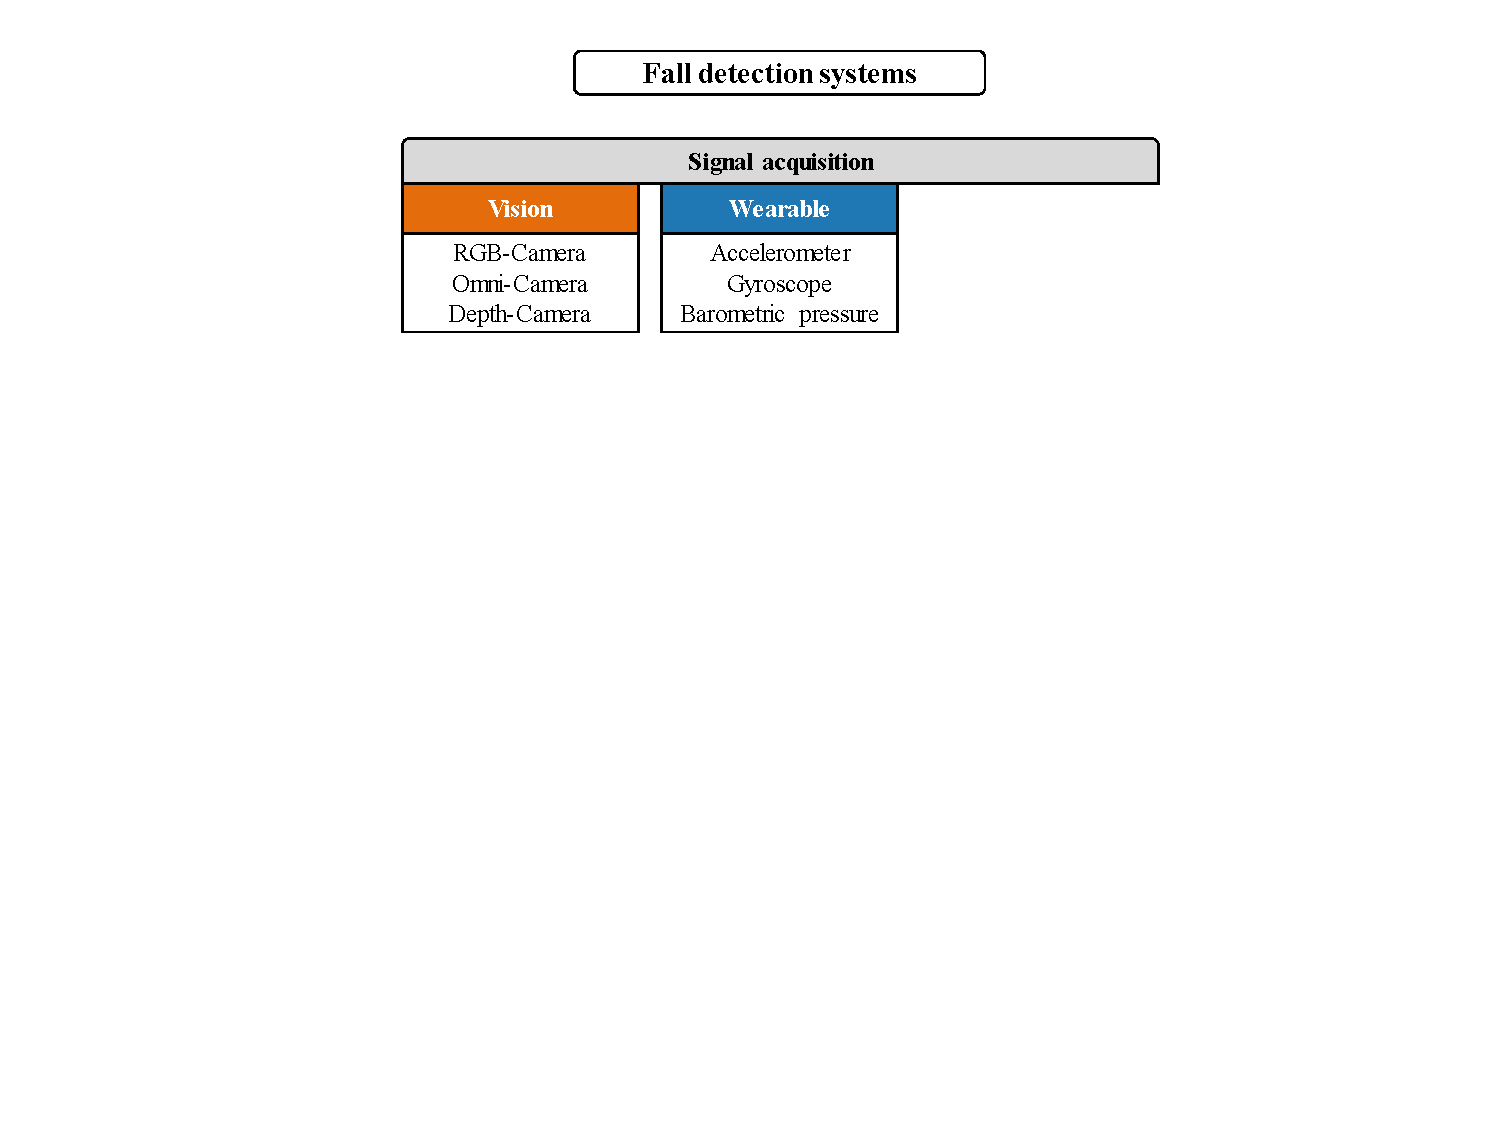
\includegraphics[width=\linewidth, trim={190 50 150 20}, clip]{fall_systems_1_2-14.pdf}
%             \onslide<4>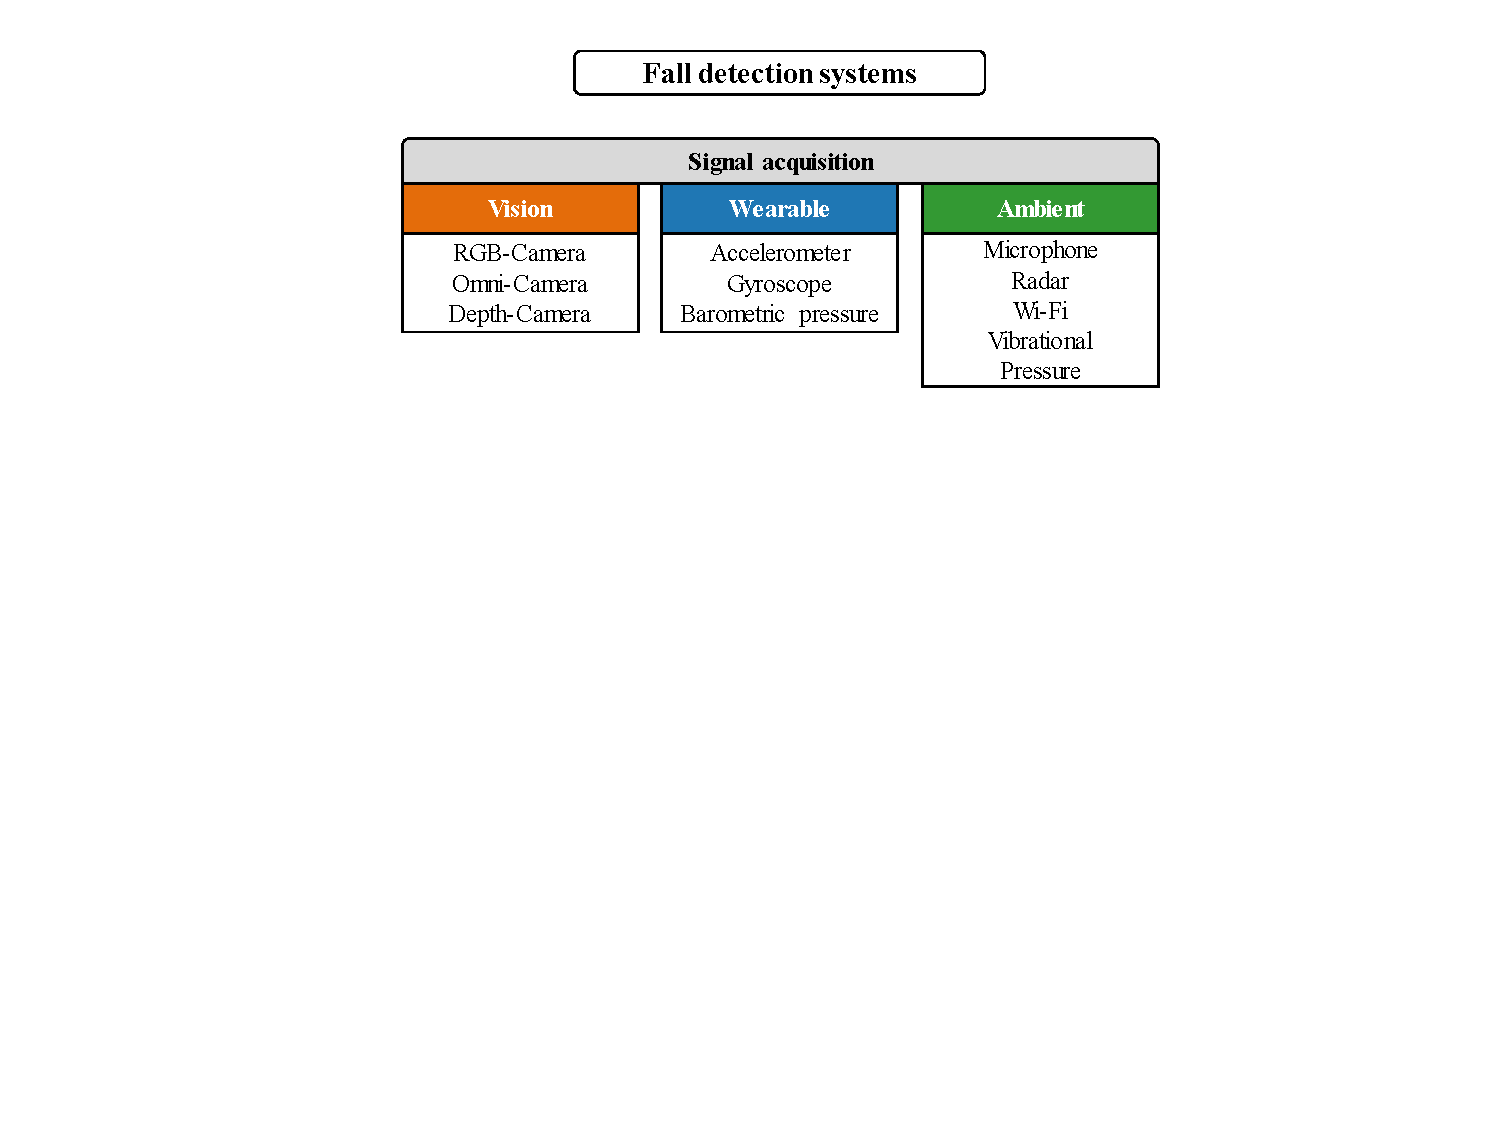
\includegraphics[width=\linewidth, trim={190 50 150 20}, clip]{fall_systems_1_3-14.pdf}
            \onslide<1>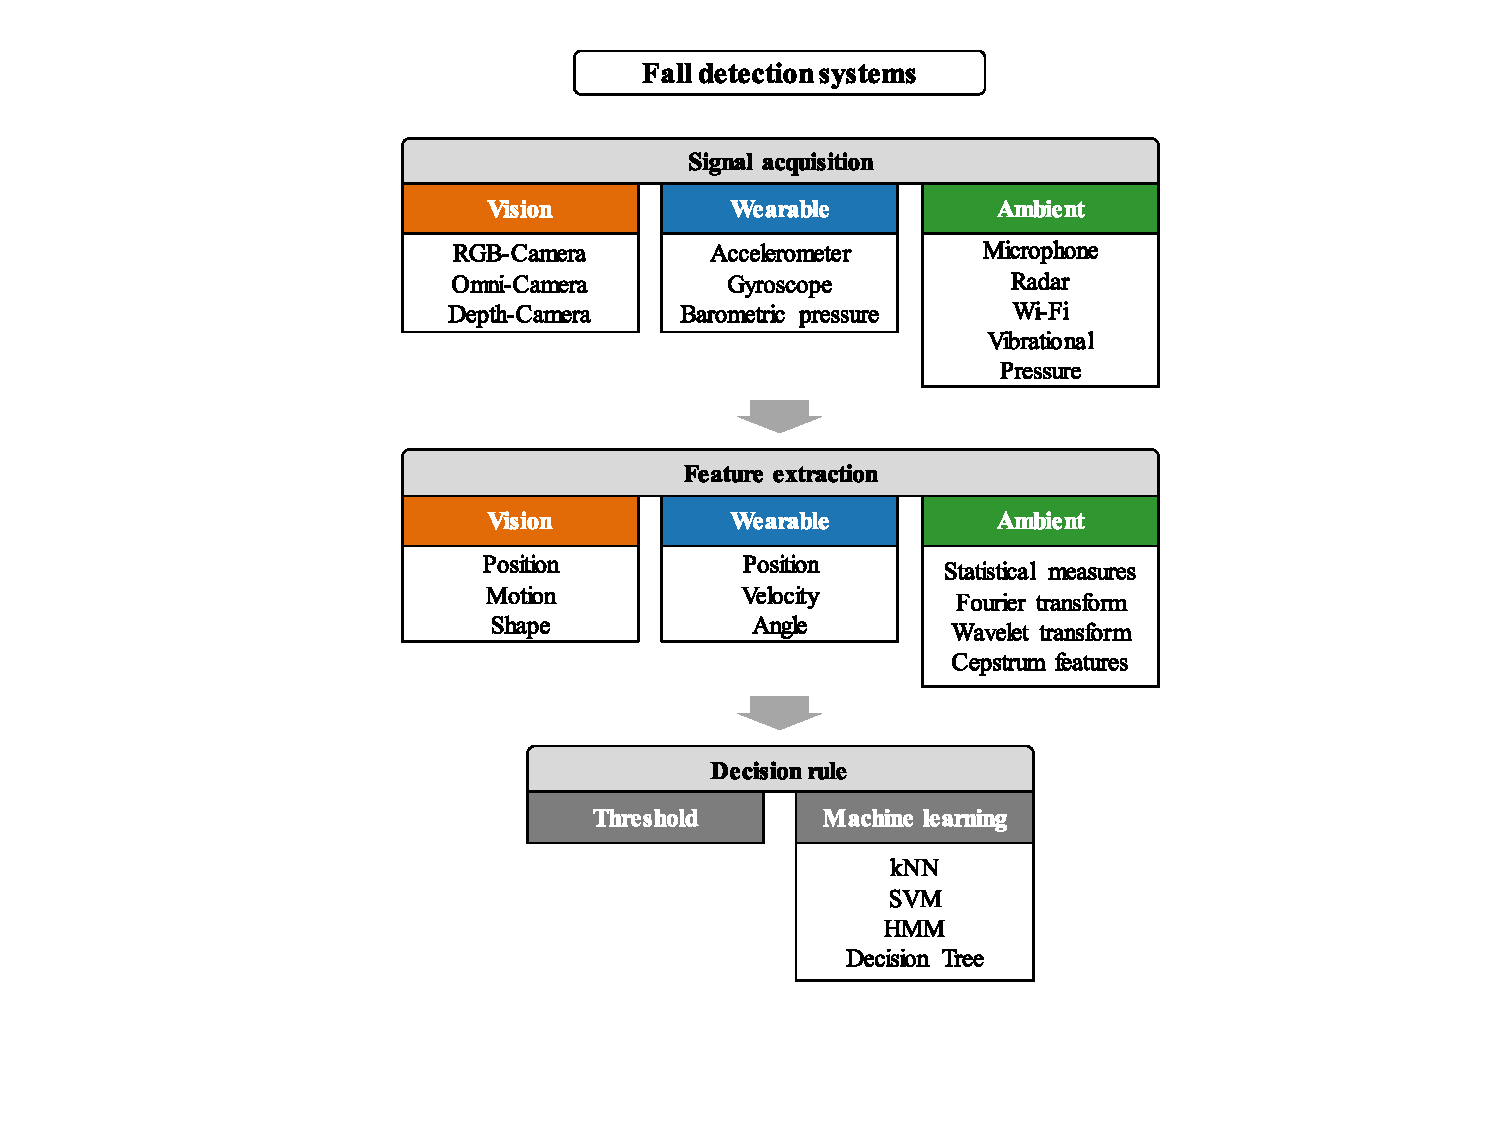
\includegraphics[width=\linewidth, trim={190 50 150 60}, clip]{fall_systems_3-14.pdf}
        \end{overprint}
    \end{minipage}
% \end{minipage}
\end{frame}




\section{Fall detection}

\begin{frame}{}
    \centering
    \vspace{3cm}
    \Huge
    \textcolor{myblue}{A fall detection system}
\end{frame}

\subsection{Tarkett sensor}
\begin{frame}{Tarkett sensor}
% \begin{figure}[ht]
\begin{minipage}[t]{0.35\linewidth}
    \vspace{0pt}
    \begin{itemize}
        \item Piezoelectric principle: $$d = \frac{Q}{F}\;,$$ (simple version) with d the \emph{piezoelectric constant}.\\
        When stressed or squeezed, the material emits charges.\\
        \pause
        \item How does this look like ?\\
            0.3 mm thick and 60 cm wide roll with customizable length
        \pause
        \item How is it installed ?\\
            \begin{itemize}
                \item Under the flooring
                \item Several connected bands for each area, hence one area corresponds to one input
            \end{itemize}

    \end{itemize}
\end{minipage}\hfill
\begin{minipage}[t]{0.64\linewidth}
    \vspace{0pt}
% \begin{minipage}{\linewidth}
    \centering
    % left bottom right top
    \onslide<1->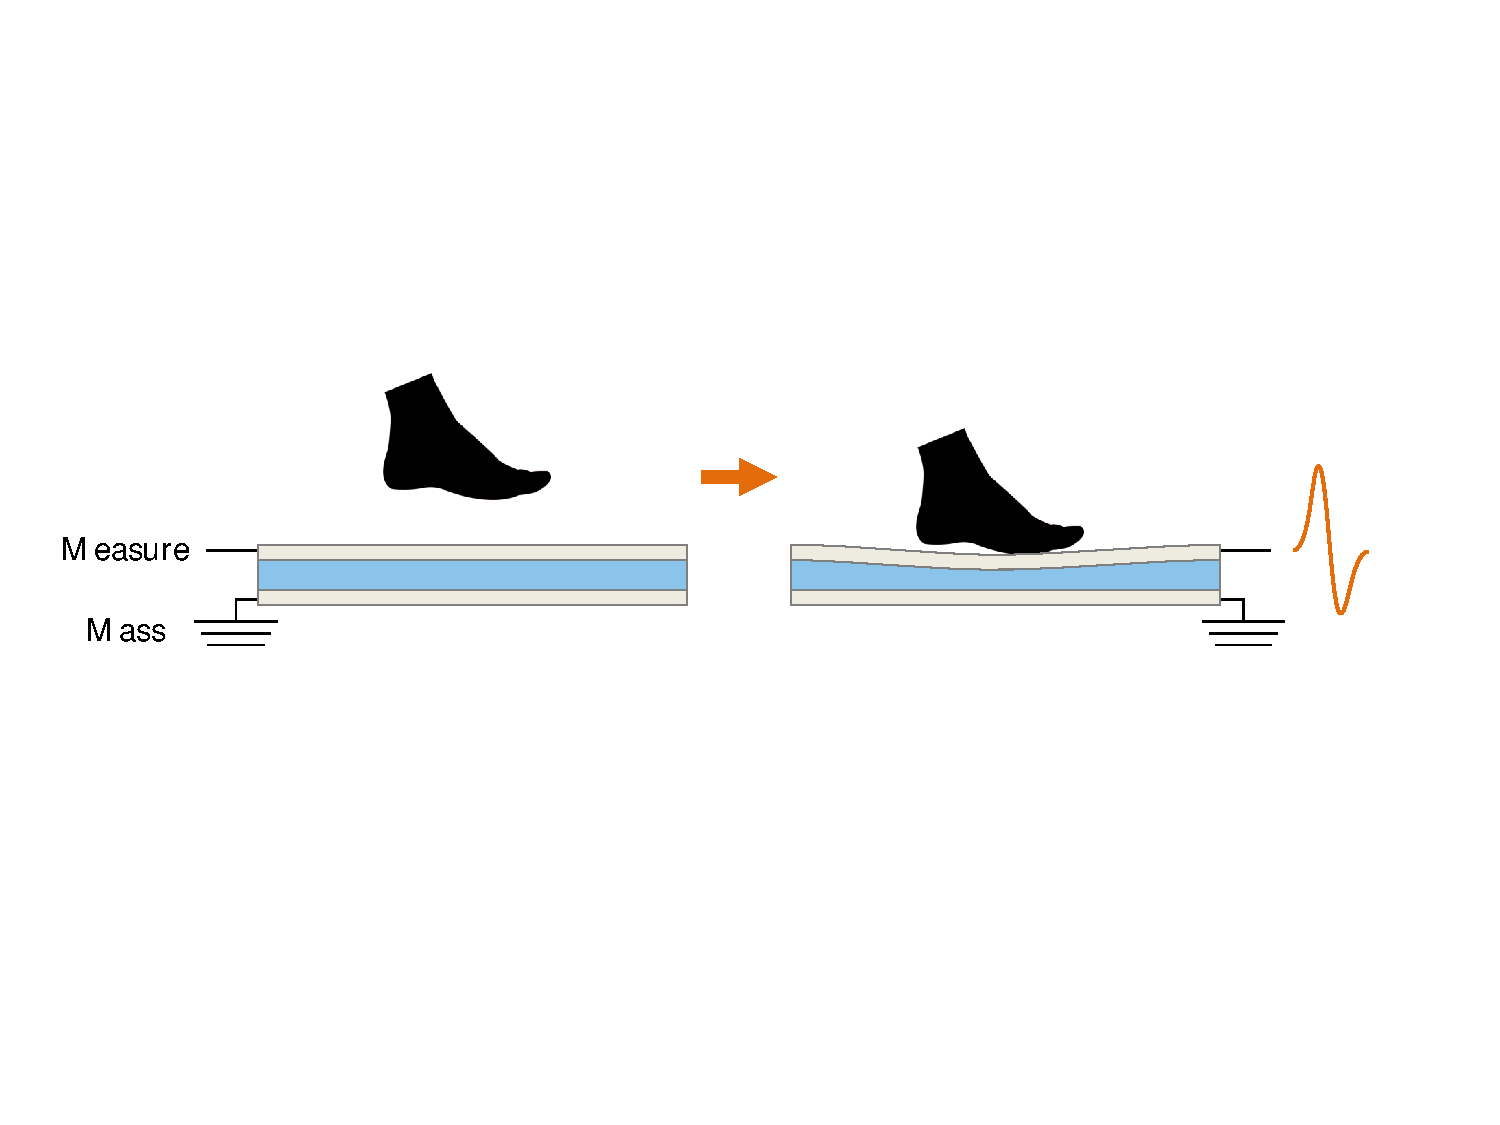
\includegraphics[width=0.9\linewidth, trim={20 220 60 170}, clip]{schema_piezo.pdf}\\
% \caption{Piezoelectric sensor principle.
%          When deformed, the piezoelectric material emits charges, hence a current can be measured in output.
%          }
% \label{fig:schema_piezoelectric}
% \end{figure}
%     \renewcommand{\ratio}{0.4}
    \begin{minipage}[t]{0.49\linewidth}
        \centering
        \onslide<2->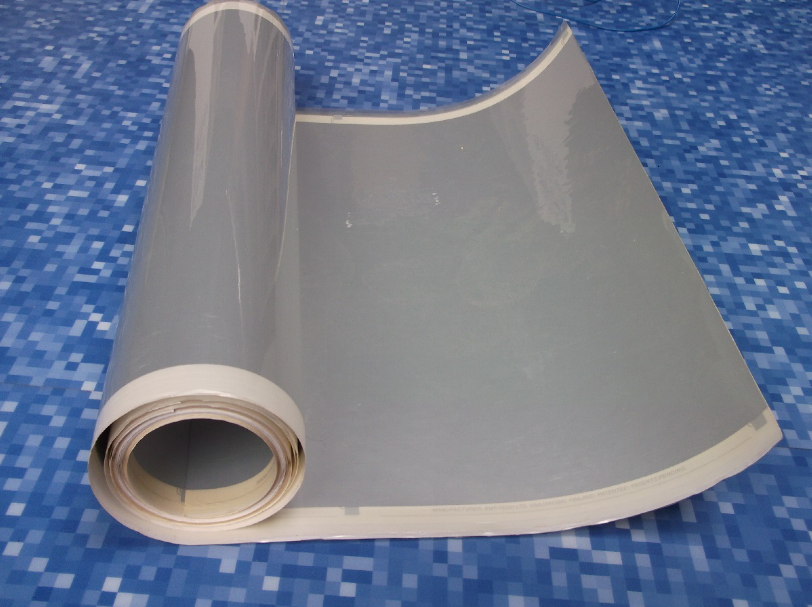
\includegraphics[width=\linewidth, height=1.9cm, keepaspectratio, trim={0 0 0 0}, clip]{photo_capteur_rouleau.png}\\
%         \small Roll of sensor
    \end{minipage}
    \begin{minipage}[t]{0.49\linewidth}
        \centering
        \onslide<2->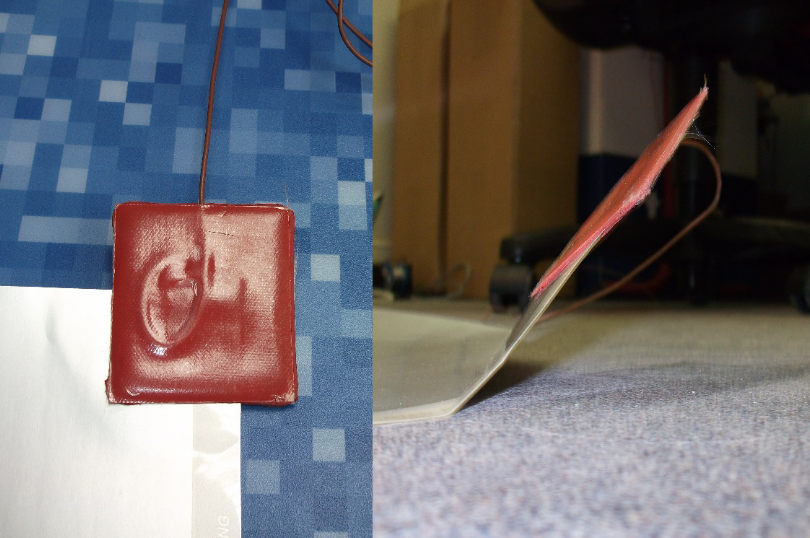
\includegraphics[width=\linewidth, height=1.9cm, keepaspectratio, trim={0 0 0 0}, clip]{photo_capteur_connecteur.png}\\
%         \small Connector
    \end{minipage}
    
% \begin{minipage}[t]{\linewidth}
    \begin{minipage}[b]{0.45\linewidth}
    \centering
    % left bottom right top
    \onslide<3->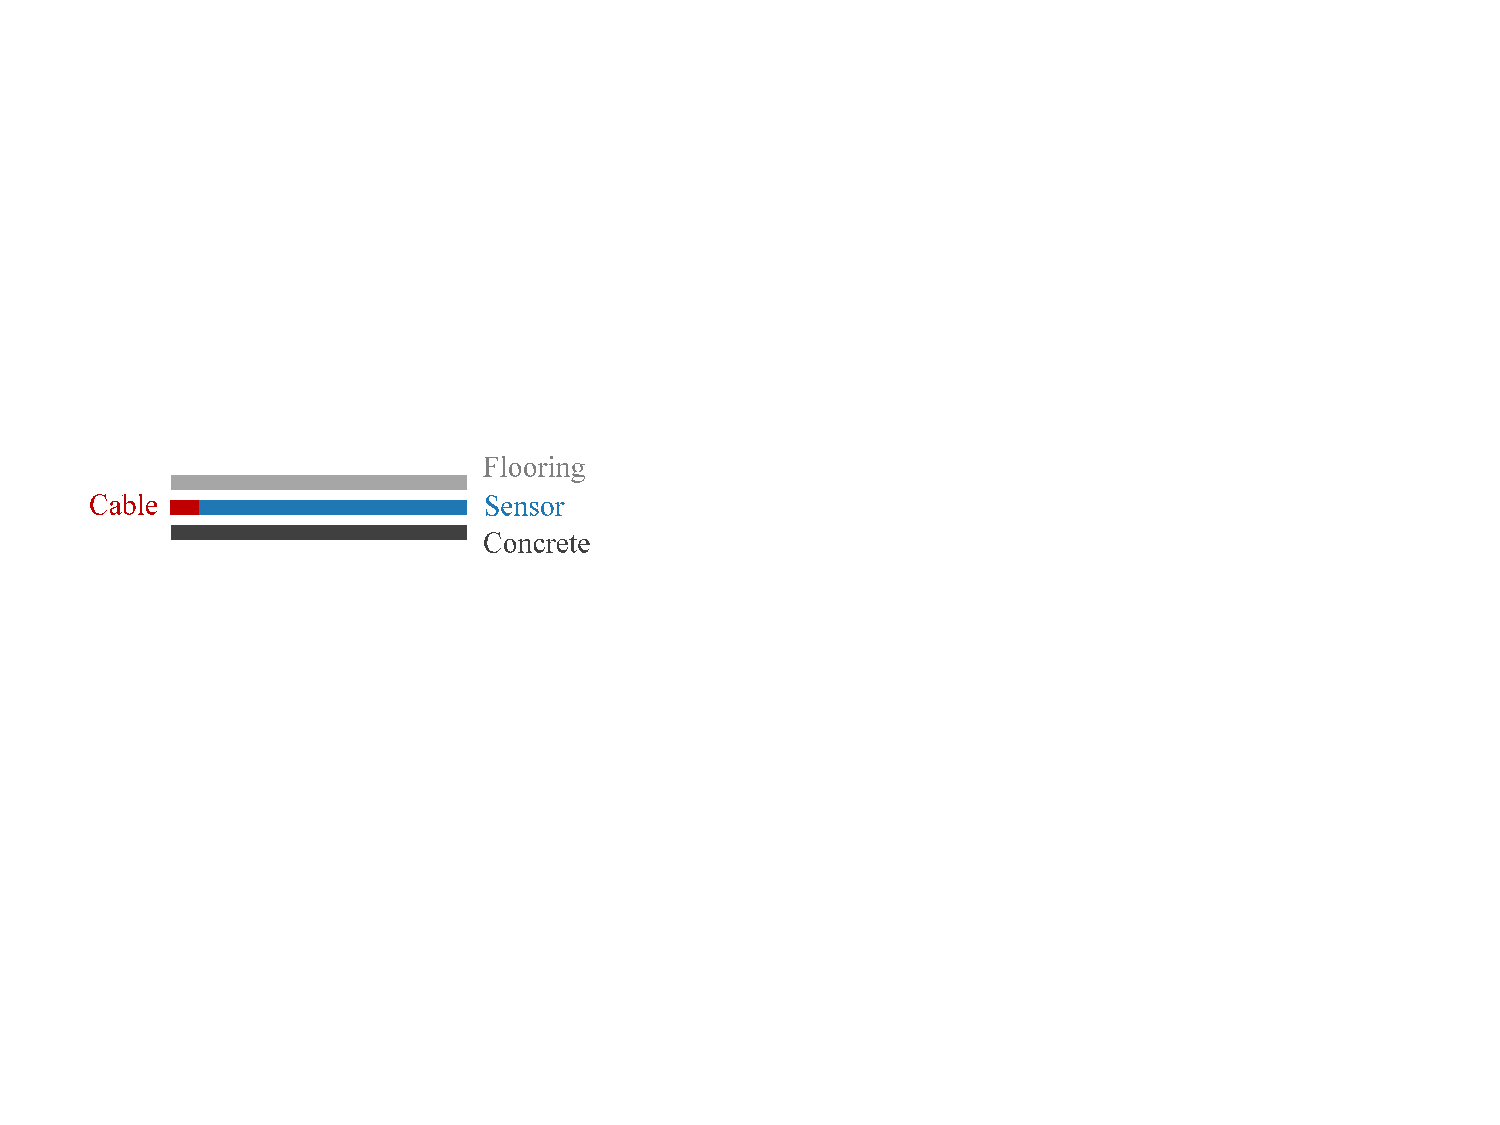
\includegraphics[width=0.95\linewidth, trim={20 260 430 200}, clip]{schema_sensor_installation_3.pdf}
    
%     \small Sensor set up
    \end{minipage}
    \hfill
    \begin{minipage}[b]{0.54\linewidth}
    \centering
    \onslide<3->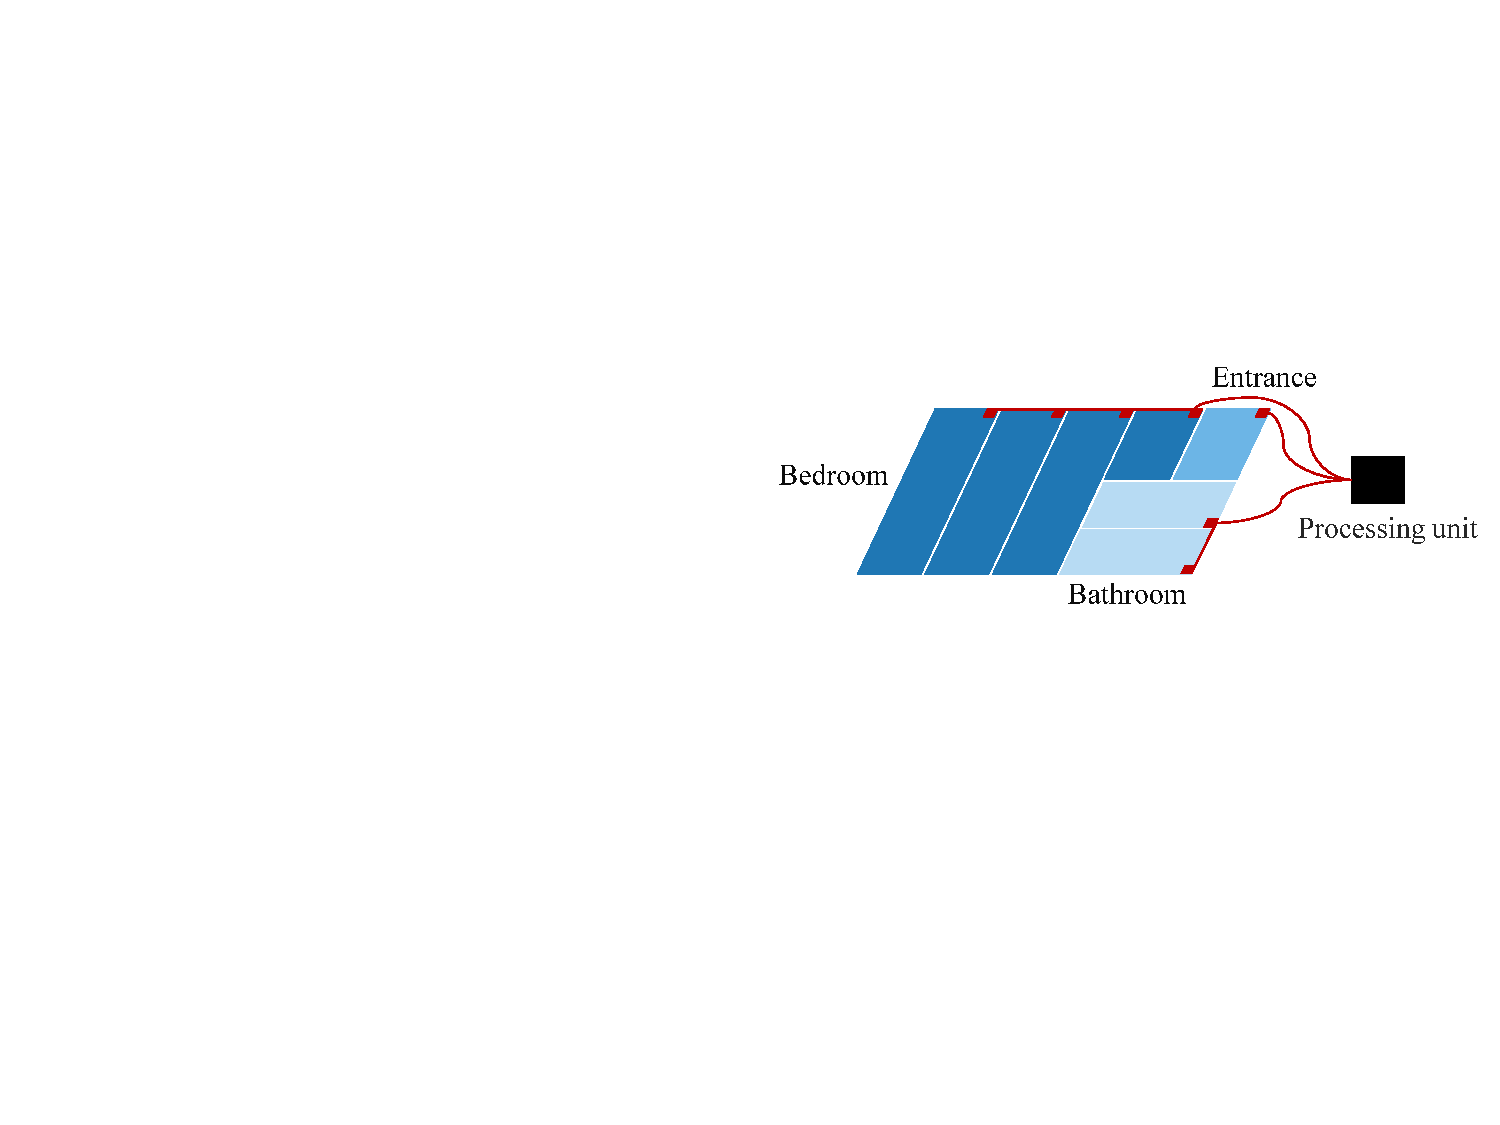
\includegraphics[width=\linewidth, trim={360 240 5 160}, clip]{schema_sensor_installation_room_3.pdf}
    
%     \small Room equipped with the system
    \end{minipage}
% \end{minipage}
\end{minipage}

\end{frame}

\subsection{Data}

\begin{frame}{Data}
\begin{minipage}[t]{0.49\linewidth}
    \vspace{0pt}
%     \begin{itemize}
        \textbf{Preprocessing}
        \begin{itemize}
            \item linear detrending
            \item low-pass filtering
            \item zeroing low energy channels
            \item sum over all channels
        \end{itemize}
%     \end{itemize}
    \medskip
    \begin{overprint}
%         \begin{minipage}{0.49\linewidth}
%         \centering
            \onslide<1>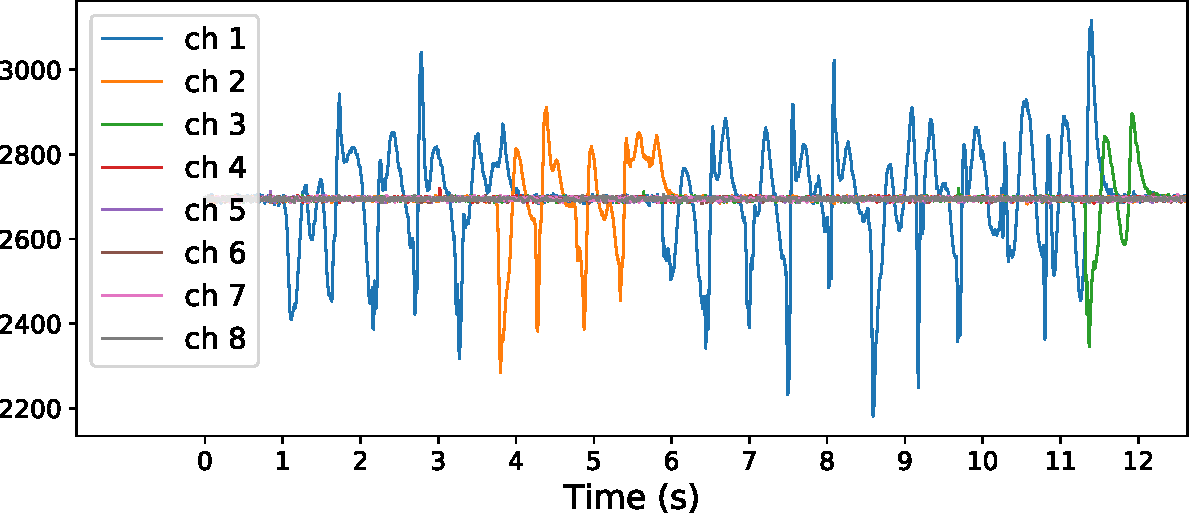
\includegraphics[trim= 0 0 0 0, width=0.8\linewidth, clip]{ex_signal_raw_2.pdf}
%             {\small Raw signal}
%         \medskip
%         \end{minipage}
%         \begin{minipage}{0.49\linewidth}
%         \centering
            \onslide<2->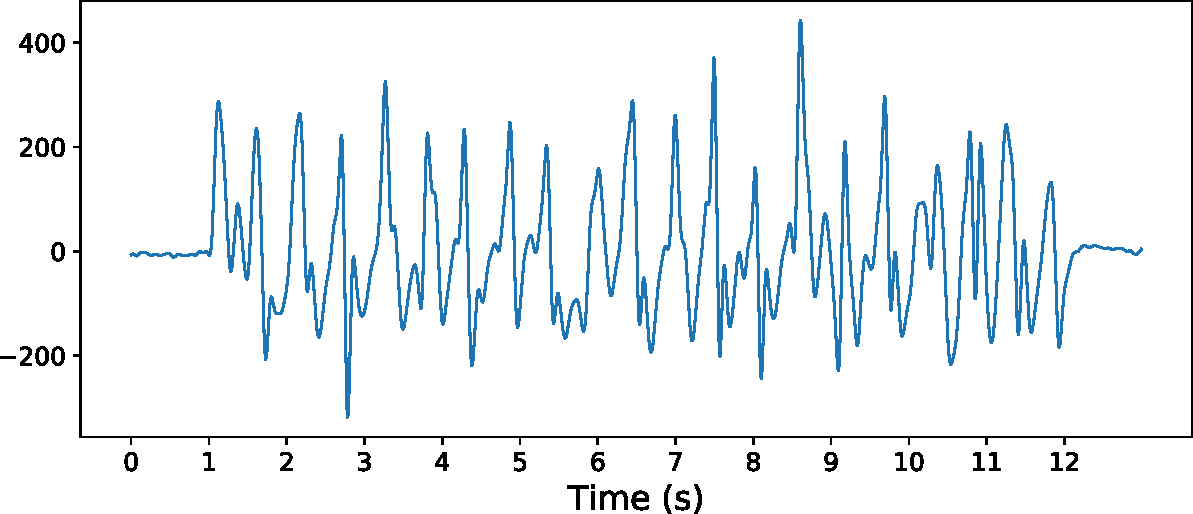
\includegraphics[trim= 0 0 0 0, width=0.8\linewidth, clip]{ex_signal_preproc_2.pdf}
%             {\small Preprocessed signal}
%         \medskip
%         \end{minipage}
    \end{overprint}
\end{minipage}\hfill
\begin{minipage}[t]{0.49\linewidth}
\vspace{0pt}
% \centering
%     \begin{itemize}
    \pause \pause
    \textbf{Experimental dataset}
    \begin{itemize}
        \item 742 signals
        \item 55\% \emph{fall}, 45\% \emph{non-fall}
        \item varied fall events (forward, backward...) and activities of daily living (walking, sitting...)
    \end{itemize}
%     \end{itemize}
    \medskip
    \centering
    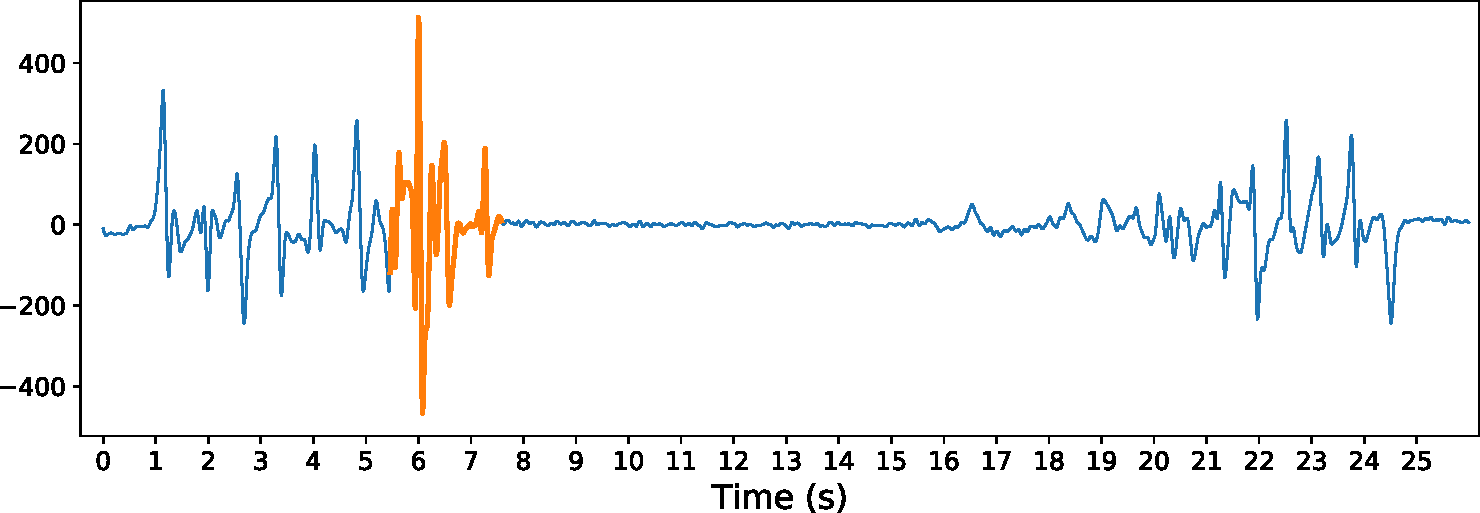
\includegraphics[width=0.85\textwidth]{ex_signal_chute_2.pdf}\\
    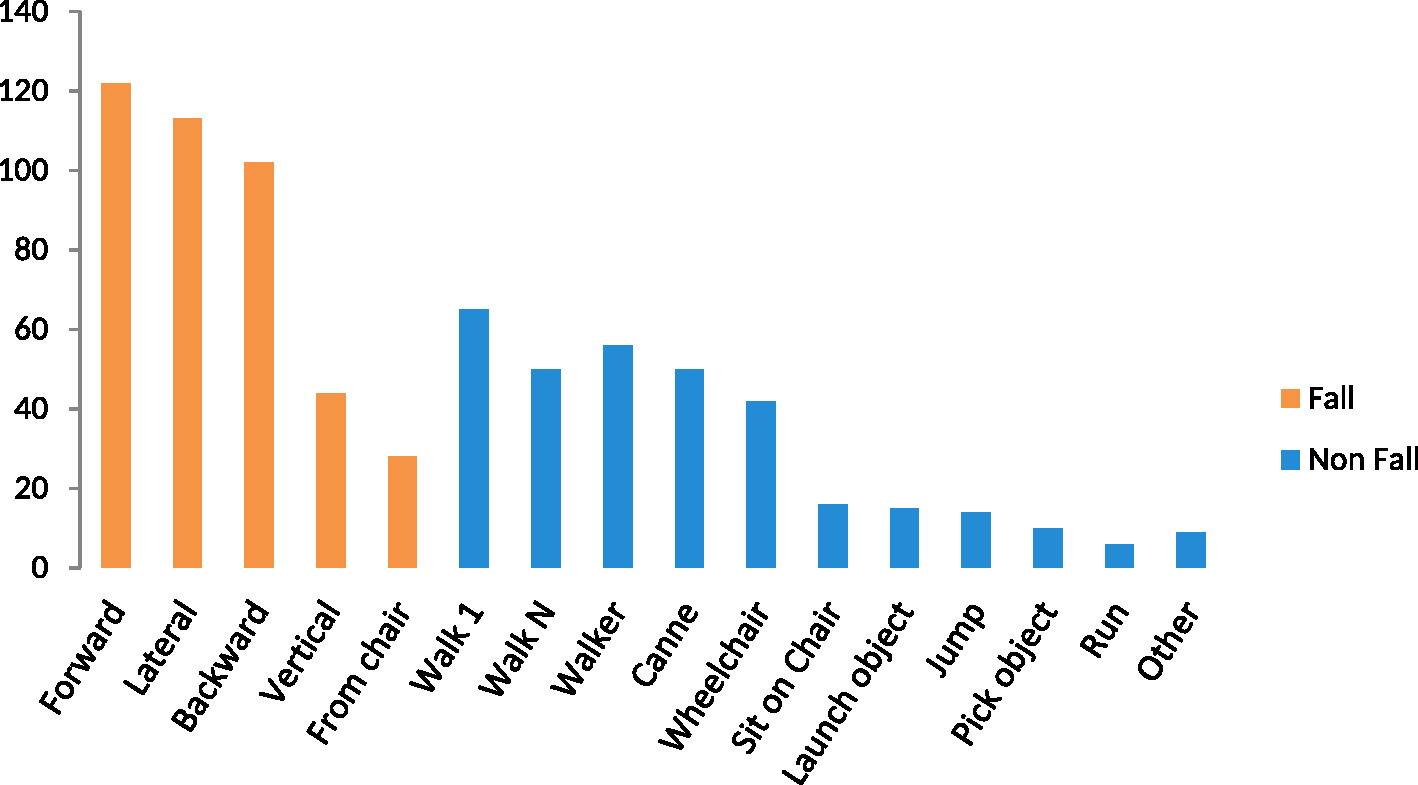
\includegraphics[width=0.8\linewidth]{exp_database_epure_2.pdf}

\end{minipage}

\end{frame}

\subsection{Method}
\begin{frame}{Method}


\begin{minipage}[t]{0.49\linewidth}
    \vspace{0pt}
Time series as \emph{feature vector}. At every timestamp:
    \begin{enumerate}
        \item Window over the signal: 2.5 s
        \item Compute feature vector: 29 statistical measures (Min, Max, Shannon energy, Percentile,...) over three representations of the signal
    \end{enumerate}
    \centering
    \begin{overlayarea}{\linewidth}{0cm}
    \centering
    \only<1>{%
    \begin{tikzpicture}[line cap=round,line join=round,>=triangle 45,x=0.2cm,y=0.4cm]
    \node[inner sep=0pt] at (0,0)
        {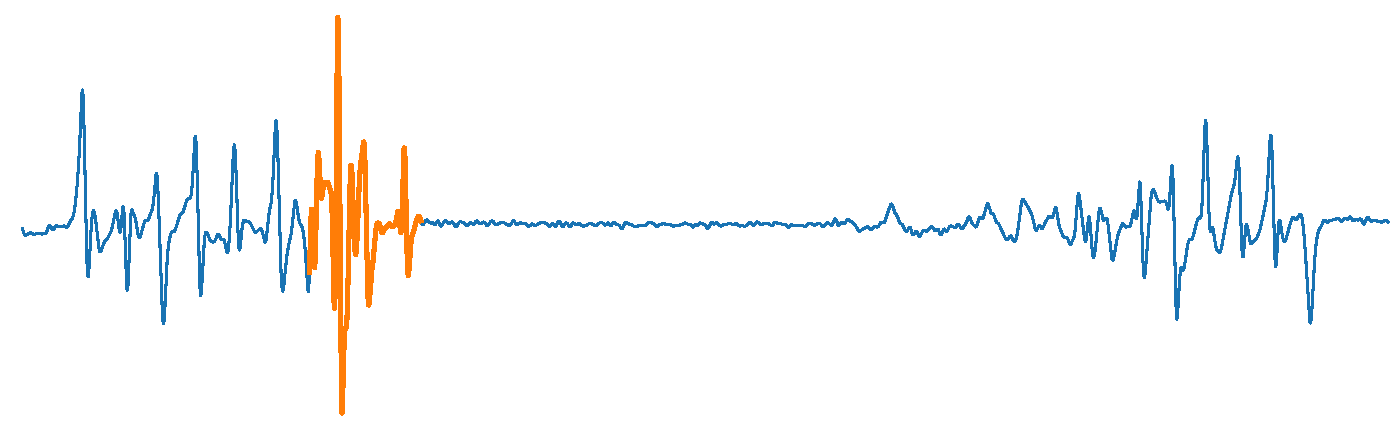
\includegraphics[width=0.55\linewidth, trim= 0 0 250 0, clip]{ex_signal_chute_2_epure.pdf}};
    \draw[color=gray!90,  line width=0.5pt] (-2.5,-2.1) rectangle (-0.5,2.2);
    \coordinate (A) at (-1.6,-2.5);
    \draw[->, >=stealth] (A) -- (-4.4,-4);
    \draw[->, >=stealth] (A) -- (-1.6,-4);
    \draw[->, >=stealth] (A) -- (1.2,-4);
    \draw (-5.5,-4.9) node[right]{$s$};
    \draw (-3.5,-4.9) node[right]{$\frac{d}{dt}s$};
    \draw (-0.5,-4.9) node[right]{$\mathcal{F}(s)$};
    \draw[->, >=stealth] (-1.6,-5.8) -- (-1.6,-6.5)
node[midway,below,yshift=-3pt]{\small Min, Max, Energy...};
    \path[draw,decorate,decoration=brace] (4.5,-7.5) -- (-7.5,-7.5)
node[midway,below,yshift=-3pt]{$\mathbf{x} \in \RR^{87}$};
    \end{tikzpicture}%
    }%
    \only<2->{%
    \begin{tikzpicture}[line cap=round,line join=round,>=triangle 45,x=0.2cm,y=0.4cm]
    \node[inner sep=0pt] at (0,0)
        {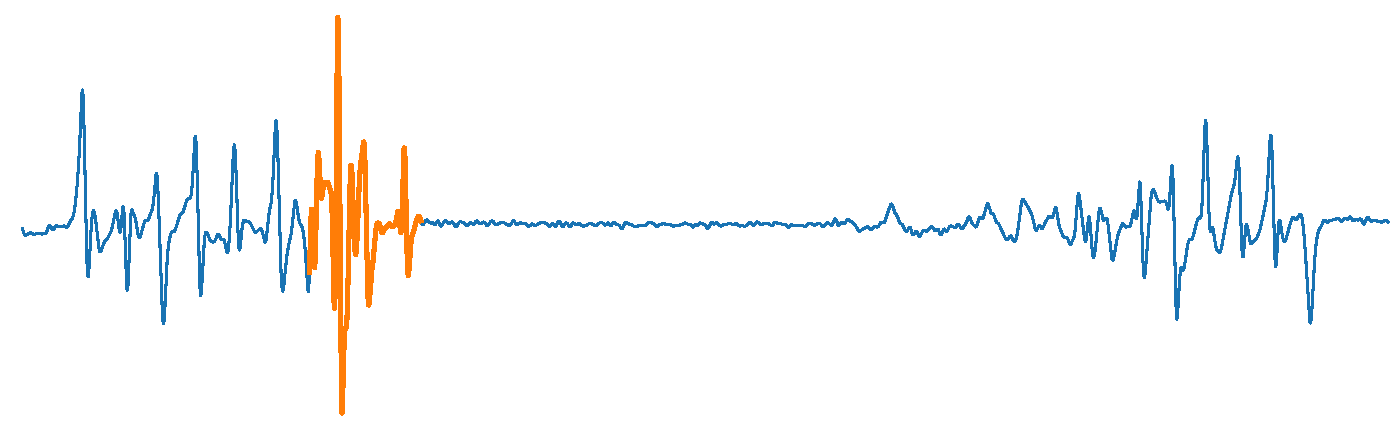
\includegraphics[width=0.55\linewidth, trim= 0 0 250 0, clip]{ex_signal_chute_2_epure.pdf}};
    \draw[color=gray!90,  line width=0.5pt] (-2.5,-2.1) rectangle (-0.5,2.2);
    \coordinate (A) at (-1.6,-2.5);
    \draw[->, >=stealth] (A) -- (-1.6,-3.5);
    \draw (-3.5,-4) node[right]{$x \in \RR^{87}$};
    \end{tikzpicture}
    }%
    \end{overlayarea}
    
    \vspace{3cm}
    \pause[3]
    \begin{enumerate}
        \item[3.] Classification model: Random Forest \cite{Breiman2001}, based on \textbf{decision trees}
        
%     \textbf{Random Forest}: Aggregation of \textbf{decision trees}.
    \end{enumerate}
\end{minipage}\hfill
\begin{minipage}[t]{0.49\linewidth}
    \vspace{0pt}
    \begin{tcolorbox}[title=Decision tree,size=title,boxrule=0.2pt]
    \small
    Feature space $\XX = \RR^Q$.
    Division of $\XX$ into non-overlapping regions $R_1,...,R_J$.
    Algorithm CART: recursive binary splits \cite{breiman84} that solve:
    \begin{gather*}
        \argmin_{X_{q}, \tau} \IG\;, \\
        \text{with} \quad \IG(X_{q}, \tau) = I(n) - \frac{N_{l}}{N_n}I(l) - \frac{N_{r}}{N_{n}}I(r)\;,\\
        \text{and} \quad I(n) = \mathrm{Gini}(n) = \sum_{k}p_{nk}(1-p_{nk})\;.
    \end{gather*}
    \end{tcolorbox}
    \begin{minipage}[t]{0.49\linewidth}
        \vspace{-5pt}
        \centering
        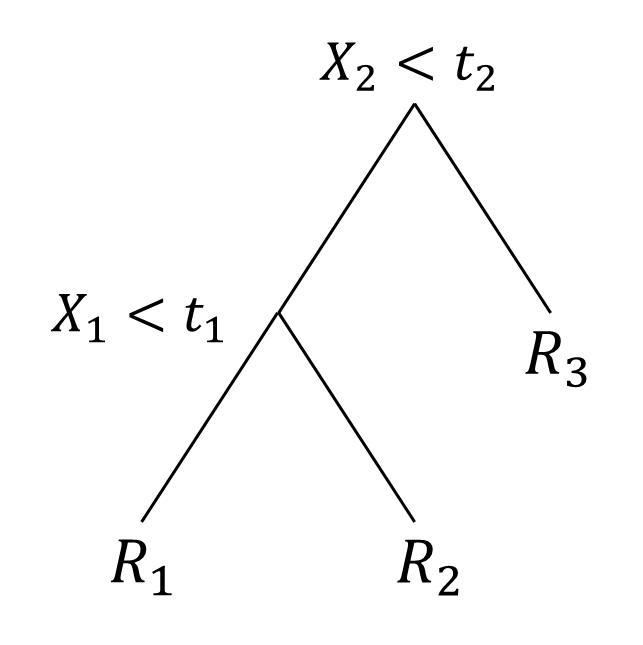
\includegraphics[width=0.65\linewidth, trim= 0 0 0 0, clip]{schema_decision_tree_1.png}\\
%     {\small Tree}
    \end{minipage}
    \begin{minipage}[t]{0.49\linewidth}
        \vspace{-5pt}
        \centering
        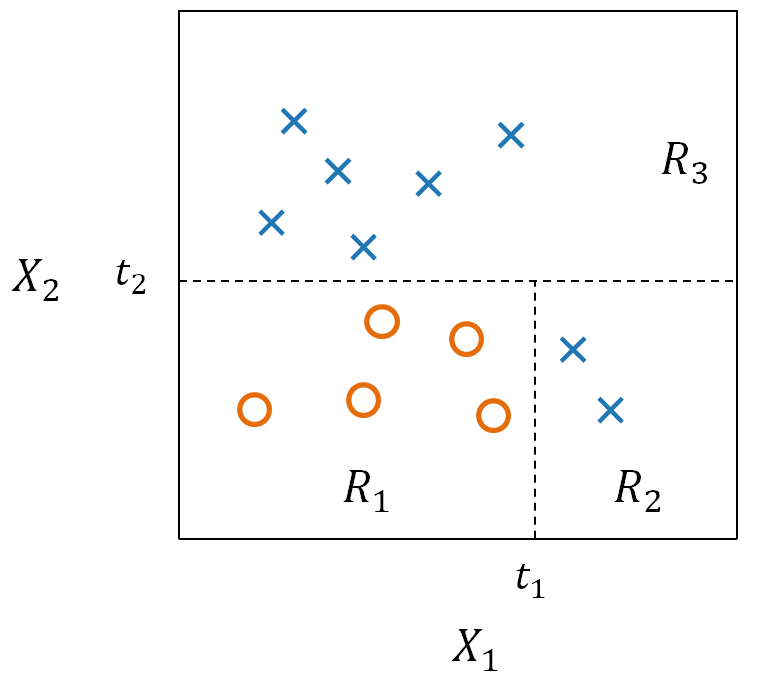
\includegraphics[width=0.9\linewidth, trim= 0 0 0 0, clip]{schema_decision_tree_3.png}\\
%     {\small Regions}
    \end{minipage}
    \centering
    \small
    Predicion function:\;
    $f(x) = \sum_{j=1}^{J}c_{j}\mathbbm{1}(x\in R_{j})$

\end{minipage}
\end{frame}

\begin{frame}{Method}
\begin{minipage}[t]{0.4\linewidth}
    \vspace{0pt}
    \begin{tcolorbox}[title=Random forest,size=title,boxrule=0.2pt]
        Decision trees $d_1,...,d_{N_T}$ grown with two rules:
        \begin{itemize}
            \item Each tree is trained with a \emph{bootstrap} of the training set
            \item At each split, access to a random subset of pool of features
        \end{itemize}
        Each tree is a ``vote'' for a class.
        The prediction function is then
        \begin{gather*}
        f(x) = \argmax_{k}f_{k}(x)\;,\\
        \text{with} \quad f_{k}(x) = \frac{1}{N_T}\sum_{i=1}^{N_T}\mathbbm{1}(d_i(x)=k)
        \end{gather*}
    \end{tcolorbox}
\end{minipage}\hfill
\begin{minipage}[t]{0.58\linewidth}
    \vspace{0pt}
%     \medskip
    \renewcommand{\ratio}{0.5}
    \begin{overlayarea}{\linewidth}{3.4cm} %{width}{height}
%     \begin{overprint}
        \only<1>{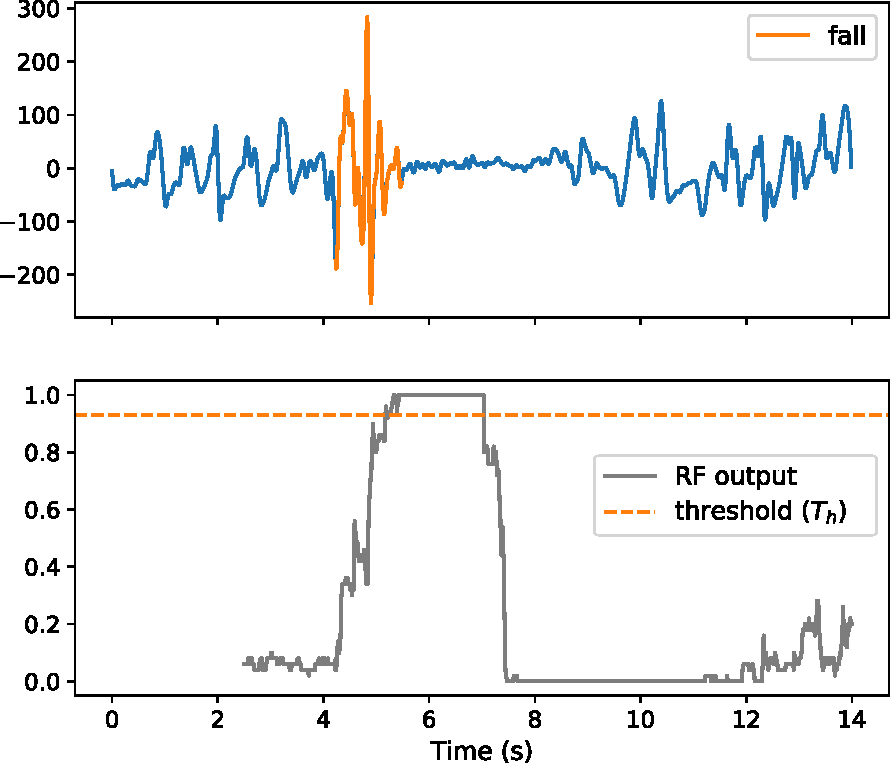
\includegraphics[width=\ratio\linewidth]{20140925a-1101-1115-FallLateral-Lateral-Yamina_begin_423_end_549_RFresponse_TP_beforebuff.pdf}}
        \only<1>{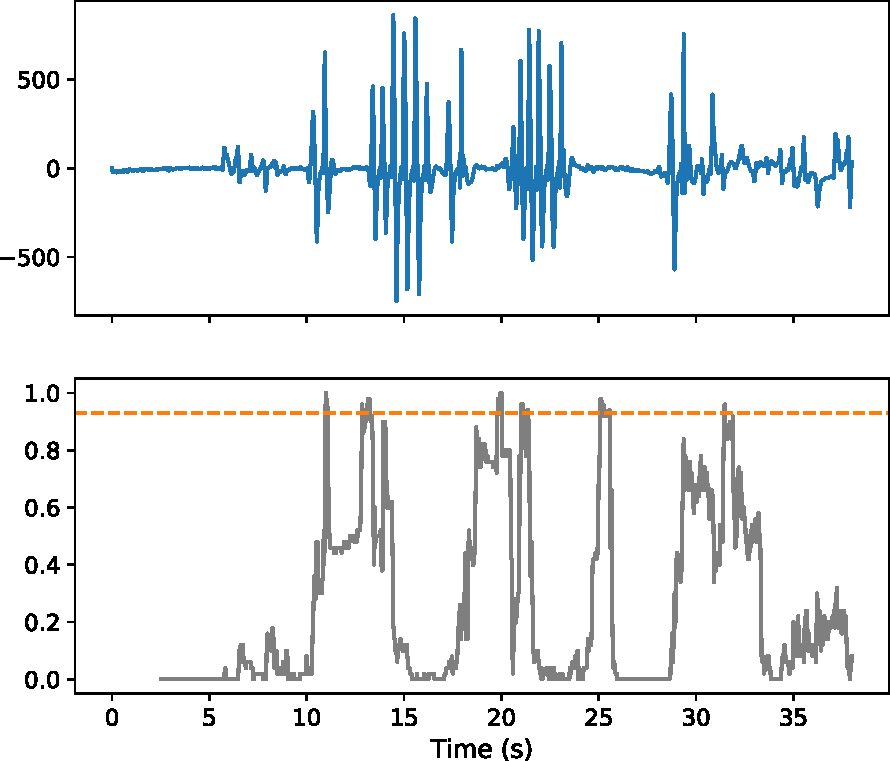
\includegraphics[width=\ratio\linewidth]{20140925a-0905-0943-Jump1-Yamina_RFresponse_TN_beforebuff_noleg.pdf}}
        \only<2->{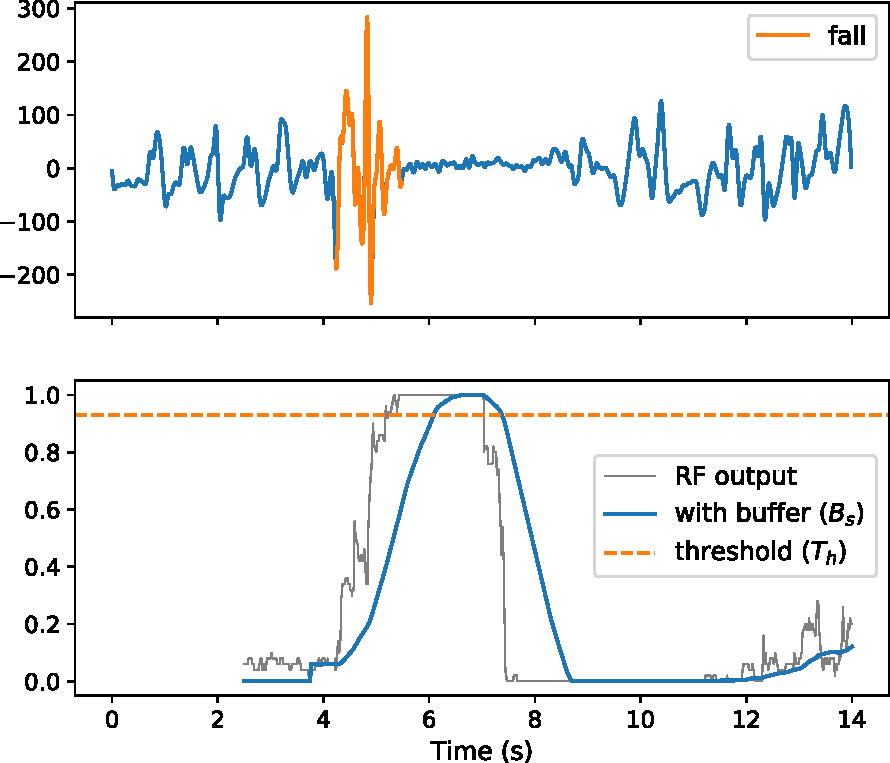
\includegraphics[width=\ratio\linewidth]{20140925a-1101-1115-FallLateral-Lateral-Yamina_begin_423_end_549_RFresponse_TP.pdf}}
        \only<2->{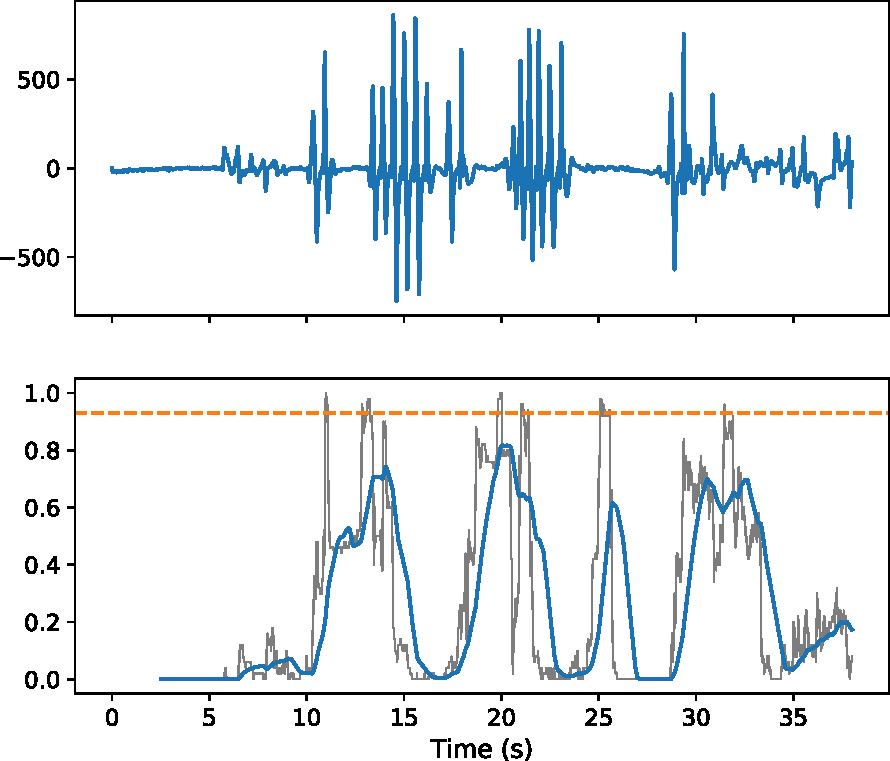
\includegraphics[width=\ratio\linewidth]{20140925a-0905-0943-Jump1-Yamina_RFresponse_TN.pdf}}
    \end{overlayarea}
%     \end{overprint}
    
    \textbf{Time aggregation}
    
    $N_f(t)$ : number of trees voting for \emph{fall}\\
    Use a buffer $B_s \in \NN$ and a threshold $T_h \in [0, 1]$
    \begin{gather*}
    g(t) = \frac{\sum\limits_{u=t-B_{s}+1}^{t}N_{f}(u)}{B_{s}\times N_{T}}\\
    \text{New binary classification function:} \quad
    d(t) = 
    \begin{cases}
    1, & \textit{if}\ g(t) > T_{h} \\
    0, & \textit{otherwise}
    \end{cases}
    \end{gather*}
\end{minipage}



\end{frame}

\begin{frame}{Method}

\begin{minipage}[t]{0.49\linewidth}
    \vspace{0pt}
    \textbf{Data augmentation}\\
    Select $r$ windows in training signals

    \centering
    \begin{tikzpicture}[line cap=round,line join=round,>=triangle 45,x=0.2cm,y=0.4cm]
    \node[inner sep=0pt] at (0,0)
        {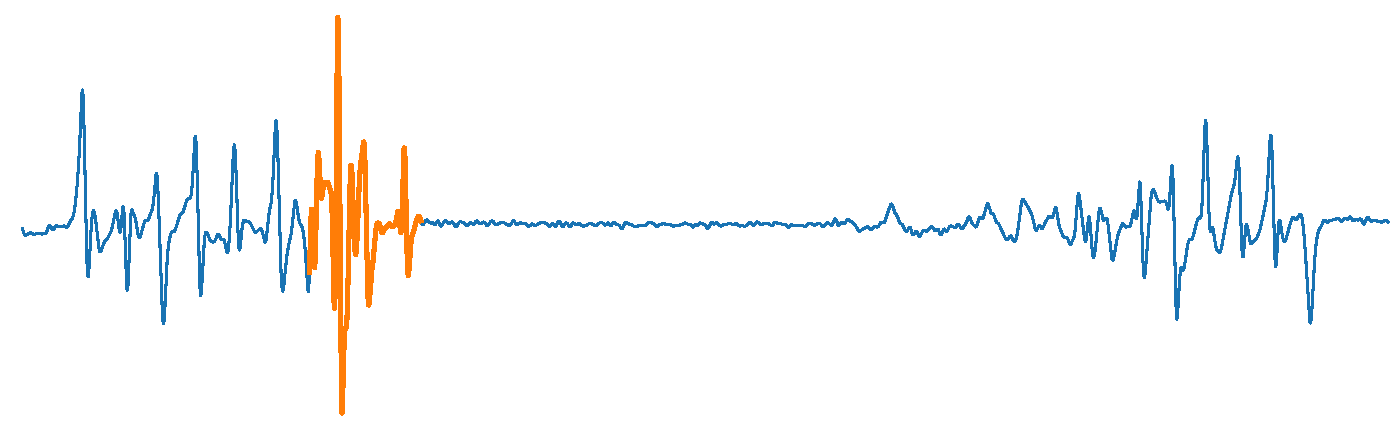
\includegraphics[width=0.55\linewidth, trim= 0 0 250 0, clip]{ex_signal_chute_2_epure.pdf}};
    \onslide<1>\draw[color=gray!90,  line width=0.5pt] (-3.3,-2.1) rectangle (-0.5,2.2);
    \onslide<2>\draw[color=gray!90,  line width=0.5pt] (-2.5,-2.1) rectangle (0.3,2.2);
    \onslide<3->\draw[color=gray!90,  line width=0.5pt] (-2.9,-2.1) rectangle (-0.1,2.2);
%     \draw (-2.5,-2.5) node[right]{$\mathbf{x} \in \RR^{87}$};
    \end{tikzpicture}
    
    \begin{overlayarea}{\linewidth}{1.25cm}
    \small
    \centering
    \only<1-3>{
    $\left[
    \begin{array}{ccc}
        x_{1,1} & ... & x_{1,Q} \\
        \onslide<2-3>{x_{2,1} & ... & x_{2,Q}} \\
        \onslide<3>{x_{3,1} & ... & x_{3,Q}} \\
    \end{array}
    \right]
    $
    }
    \only<4->{
    $\left[
    \begin{array}{ccc}
        x_{1,1} & ... & x_{1,Q} \\
        \vdots & & \vdots \\
        x_{r,1} & ... & x_{r,Q} \\
    \end{array}
    \right]
    $
    }
    \end{overlayarea}
    
%     \pause
%     \pause \pause \pause \pause
    \only<5->{
    \raggedright
    \textbf{Feature reduction}
    \begin{tcolorbox}[title=Feature importance,size=title,boxrule=0.2pt]
        \begin{gather*}
        \text{Tree: } I(X_{q}) = \sum_{\text{nodes}\ t}p(t)\Delta i(t)\mathbbm{1}(v(t)=X_{q})\\
        \text{Random forest: }I(X_{q}) = \frac{1}{N_{T}}\sum_{n=1}^{N_T}I(T_n, X_{q})
        \end{gather*}
    \end{tcolorbox}
    }
\end{minipage}\hfill
\begin{minipage}[t]{0.49\linewidth}
    \vspace{0pt}
    \begin{overlayarea}{\textwidth}{\textheight}
    \only<5>{
    \centerline{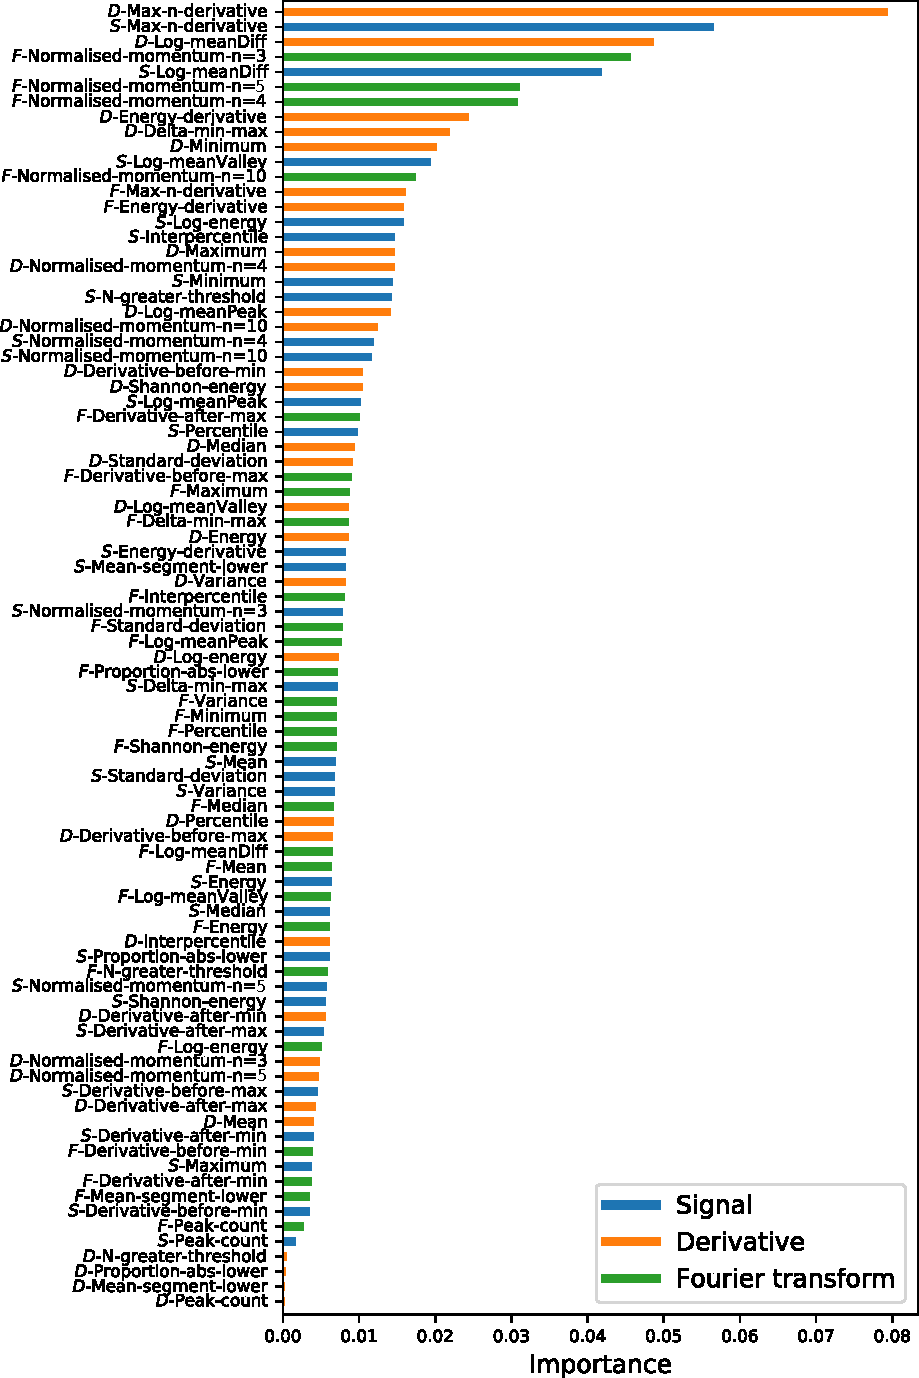
\includegraphics[width=0.75\linewidth, trim= 0 0 0 0, clip]{plot_feature_importance_all_epure.pdf}}
    }
    \only<6->{
    \begin{tcolorbox}[title=Recursive feature elimination,size=title,boxrule=0.2pt]
    Initial pool of $Q$ features $X_1, ..., X_Q$.
        \begin{enumerate}
            \item Train several times and record variable importances
            \item Average of importances over trainings. $X_{q}* = \argmin_{X_i} I(X_{i})$
            \item Remove $X_{q}*$ from the pool of features and back to step 1
        \end{enumerate}
    \end{tcolorbox}
    \smallskip
    \centerline{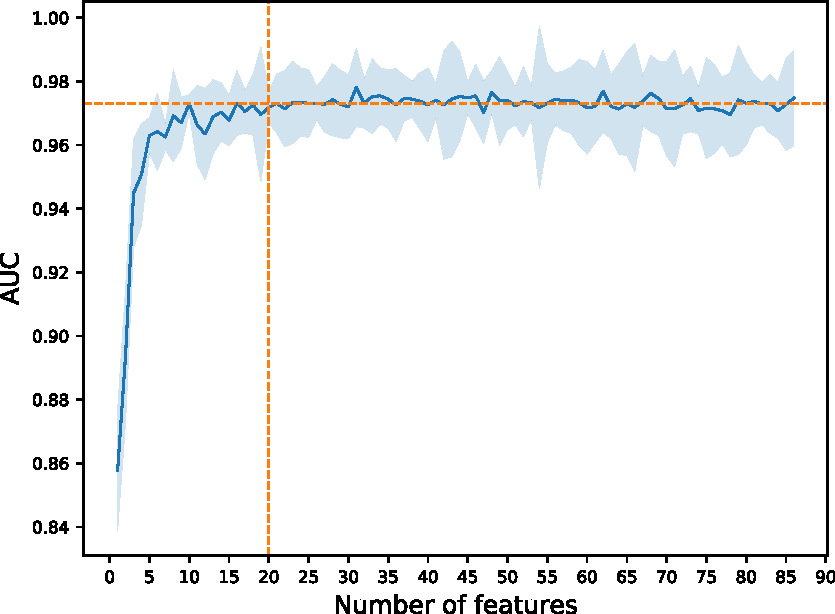
\includegraphics[width=0.7\linewidth]{plot_rf_feat_reduc_AUC_epure.pdf}}

    }
    \end{overlayarea}
\end{minipage}
\end{frame}

\subsection{Results}
\begin{frame}{Results}
    \renewcommand{\ratio}{0.32}
    \centering
    \begin{minipage}[t]{0.9\linewidth}
        \centering
        \begin{minipage}[t]{\ratio\linewidth}
            \centering
            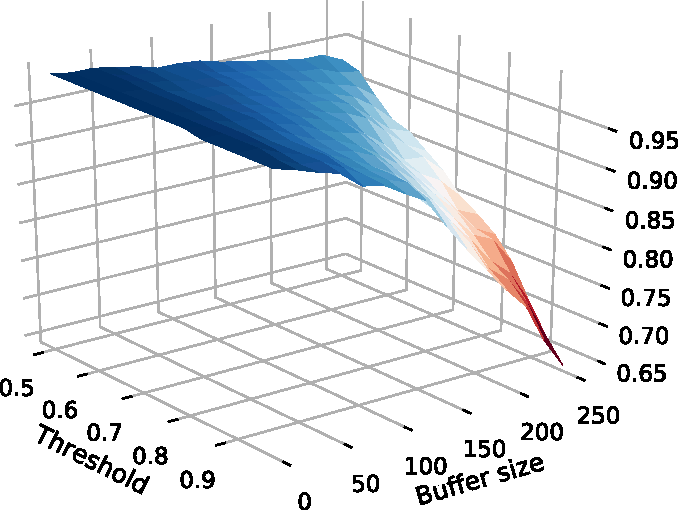
\includegraphics[width=\linewidth]{plot3d_compare_methods_buff_2019_12_05_14h51m35s_rf_TPR_view2.pdf}\\
            \smallskip
            {\small True positive rate}
        \end{minipage}
        \begin{minipage}[t]{\ratio\linewidth}
            \centering
            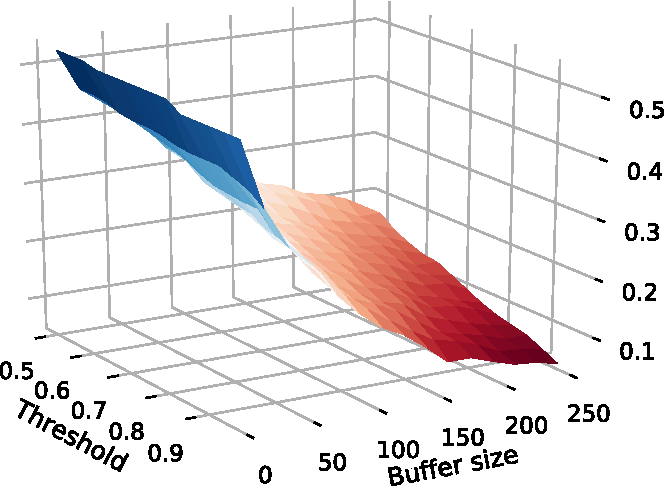
\includegraphics[width=\linewidth]{plot3d_compare_methods_buff_2019_12_05_14h51m35s_rf_FPR_view2.pdf}\\
            \smallskip
            {\small False positive rate}
        \end{minipage}
        \begin{minipage}[t]{\ratio\linewidth}
            \centering
            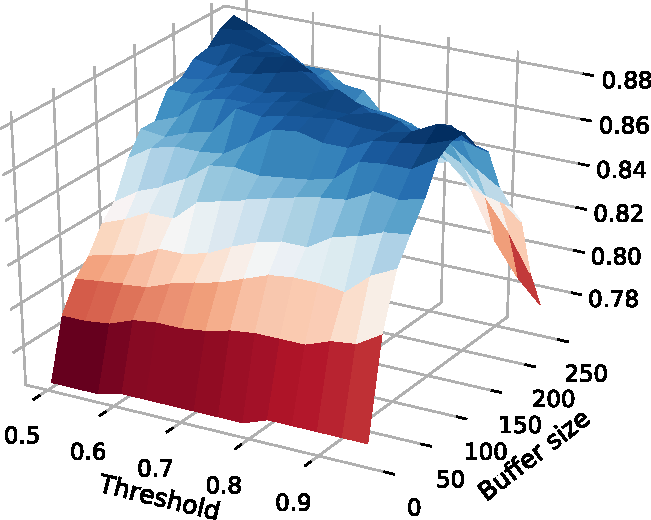
\includegraphics[width=0.92\linewidth]{plot3d_compare_methods_buff_2019_12_05_14h51m35s_rf_Accuracy.pdf}\\
            \smallskip
            {\small Accuracy}
        \end{minipage}
    \end{minipage}

\medskip

\begin{table}[ht]
\small
\begin{center}
\begin{tabular}{c c c c c c}
\toprule
  Model     & $\Acc$ & $\TPR$ & $\FPR$ & $\TPR_{\text{min}}^{\FPR<10}$ & $\TPR_{\text{max}}^{\FPR<10}$ \\
\midrule
 \multicolumn{6}{c}{\footnotesize $r = 5,\; Q = 20$} \\
\hline
LR   &  86.8 $\pm$ 1.5 & 90.5  $\pm$  2.4 &  17.7  $\pm$  4.9 & 67.0  $\pm$  10.8 & 80.4 $\pm$  6.4 \\
LDA   &  85.5  $\pm$  1.2  & 91.0  $\pm$  2.1 &  21.7  $\pm$  3.7 & 56.9  $\pm$  7.0 & 78.7  $\pm$  3.8 \\
k-NN  &    87.0  $\pm$  1.9 & 89.2  $\pm$  1.4  & \textbf{16.0  $\pm$  4.7} & 63.1  $\pm$  4.2 & 83.1  $\pm$  2.5 \\
SVM  &   87.6  $\pm$  3.2 & 90.0  $\pm$  4.5 & \textbf{15.5  $\pm$  6.8} & 69.2 $\pm$ 2.1 & 82.9  $\pm$  3.2 \\
MLP  &\textbf{88.2  $\pm$  1.5} & \textbf{92.4  $\pm$  1.2} & 17.3  $\pm$  4.1 & 71.4  $\pm$  4.5 & 85.1  $\pm$  2.1\\
RF  & \textbf{88.2  $\pm$  1.5} & \textbf{91.7 $\pm$ 3.5} & 16.2  $\pm$  6.2 & 63.8  $\pm$  6.8 & 84.3  $\pm$  7.9 \\
% \hline
%  \multicolumn{6}{c}{\rule{0pt}{12pt} \footnotesize $r = 10,\; Q = 30$} \\
% \hline
% LR   & 87.5  $\pm$  2.5 & 93.4  $\pm$  2.3 & 20.0  $\pm$  4.2  & 66.5  $\pm$  2.4 & 83.1  $\pm$  1.9 \\
% LDA   & 86.4  $\pm$  1.3  & 89.5  $\pm$  2.3  & 17.5  $\pm$  2.6 & 56.7  $\pm$  4.2 & 76.8  $\pm$  3.7\\
% k-NN  & 87.8  $\pm$  4.1  & 90.7  $\pm$  4.3  & 16.0  $\pm$  4.7 & 63.8  $\pm$  5.3 & 80.7  $\pm$  4.5 \\
% SVM  &  88.3  $\pm$  3.4  & 88.0  $\pm$  4.2 & \textbf{11.3  $\pm$  4.0} & 68.7  $\pm$  5.7 & 85.3  $\pm$  4.7 \\
% MLP  & \textbf{89.8  $\pm$  1.8} & \textbf{95.4  $\pm$  1.2} & 17.2  $\pm$  3.6 & 72.1  $\pm$  4.8 & 88.3  $\pm$  1.6 \\
% RF  & \textbf{89.9  $\pm$  2.5} & \textbf{93.6  $\pm$  2.5} & \textbf{15.0  $\pm$  3.0} & 62.6  $\pm$  3.8 & 85.1  $\pm$  2.9 \\
\bottomrule
\end{tabular}
\end{center}
\end{table}

\end{frame}